\documentclass{article}

% Just to have them already
% \begin{sloppypar}
% \end{sloppypar}


% Just try to parse, do not ask for input
\nonstopmode

% Bibliography
\usepackage{natbib}
\bibpunct{(}{)}{;}{a}{}{;}

% Use 'It was found that A is B (Name 1234)' style
\setcitestyle{authoryear,open={},close={}}

% Affiliations
\usepackage{authblk}
\title{
  Transmembrane helices are also 
  an overlooked source of major histocompatibility complex class II epitopes
  and evolutionary more conserved than expected by chance
}
\author[1]{Richèl J.C. Bilderbeek}
\author[1]{Maxim Baranov}
\author[1]{Geert van den Bogaart}
\author[1]{Frans Bianchi}
\affil[1]{GBB, University of 
Groningen, Groningen, The Netherlands}

% Use double spacing
\usepackage{setspace}
\doublespacing

\usepackage{listings}
\usepackage{hyperref}
\usepackage{todonotes}
\usepackage{verbatim}
\usepackage{pgf}
\usepackage{bm}
\usepackage{multirow}
\usepackage{amsfonts}
\usepackage{array}
\usepackage{booktabs}
\newcolumntype{C}[1]{>{\centering\arraybackslash}p{#1}}
\newcolumntype{L}[1]{>{\raggedright\arraybackslash}p{#1}}
\usepackage{longtable}

\usepackage{tkz-graph}
\usetikzlibrary{arrows,automata}
\usetikzlibrary{calc}
\usetikzlibrary{arrows.meta}

% sidewaysfigure
\usepackage{rotating}

% Style of listings
% From http://r.789695.n4.nabble.com/
%   How-to-nicely-display-R-code-with-the-LaTeX-package-listings-tp4648110.html
\usepackage{fancyvrb} 
\definecolor{codegreen}{rgb}{0,0.6,0}
\definecolor{codegray}{rgb}{0.5,0.5,0.5}
\definecolor{codepurple}{rgb}{0.58,0,0.82}
\definecolor{backcolor}{rgb}{0.95,0.95,0.92}
\lstdefinestyle{mystyle}{
  language=R,% set programming language
  basicstyle=\ttfamily\small,% basic font style
  commentstyle=\color{gray},% comment style
  numberstyle=\scriptsize,% use small line numbers
  numbersep=10pt,% space between line numbers and code
  tabsize=2,% sizes of tabs
  showstringspaces=false,
  captionpos=b,% positioning of the caption below
  breaklines=true,% automatic line breaking
  escapeinside={(*}{*)},% escaping to LaTeX
  fancyvrb=true,% verbatim code is typset by listings
  extendedchars=false,% prohibit extended chars (chars of codes 128--255)
  alsoletter={.<-},% becomes a letter
  alsoother={$},% becomes other
  otherkeywords={!=, ~, $, \&, \%/\%, \%*\%, \%\%, <-, <<-, /},
  deletekeywords={c}% remove keywords 
}
\lstset{style=mystyle}

% Adds numbered lines. Not yet...
% \usepackage{lineno}
% \linenumbers

%comments
\newcommand{\frans}[1]{\textcolor{blue}{\textbf{[FB: #1]}}}
\newcommand{\richel}[1]{\textcolor{orange}{\textbf{[RB: #1]}}}

\begin{document}

\maketitle

\begin{abstract}

Transmembrane helices (TMHs) in the human proteome
are an overrepresented potential source of epitopes on major 
histocompatibility complex (MHC) class I for the majority of HLA-I haplotypes. 
It is unknown if the immune system is as able to detect 
TMHs as found in pathogens.
Additionally, it is unknown if MHC-II is also likelier to detect
human and pathogen TMHs than expected by chance.
It is unknown if natural selection is the cause that 
the immune system is more attentive for TMHs
This study shows that MHC-I [also has/does not have] more
epitopes derived from a TMH for a pathogen proteome, when compared with
a host proteome.
Additionally, MHC-II binds to polypeptides derived from TMHs 
[less/equally/more] often than expected by chance.
Lastly, using an innovative computation method, 
we show that natural selection on TMHs is [strong enough/still too weak]
to detect.
Our findings suggest that the immune system is [less/neutral/more]
vigilant to TMHs than expected by chance and this has 
left [a clear/a weak/no]
signal in the evolutionary history of the pathogen.

\end{abstract}

{\bf Keywords:} antigen presentation, membrane proteins, bioinformatics, 
adaptive immunity, transmembrane domain, epitopes, T lymphocyte, 
MHC-1, MHC-I, MHC-2, MHC-II, COVID-19

%%%%%%%%%%%%%%%%%%%%%%%%%%%%%%%%%%%%%%%%%%%%%%%%%%%%%%%%%%%%%%%%%%%%%%%%%%%%%%%%
\section{Introduction}
%%%%%%%%%%%%%%%%%%%%%%%%%%%%%%%%%%%%%%%%%%%%%%%%%%%%%%%%%%%%%%%%%%%%%%%%%%%%%%%%

\paragraph{Immune response}

Our immune system fights invaders on a daily basis.
These invaders can be fungi, bacteria or viruses.
The innate immune response is its first general 
and immediate strategy, where the acquired immune response
needs time to develop its specialized and more effective
combat forces.

\paragraph{Immune response by MHC-I}

All nucleated cells in humans present randomly sampled polypeptides
fragments to the surroundings of the cell using the Major 
Histocompatibility Complex (MHC) class I molecules.
If a cell gets infected by a virus, also the virus' polypeptides
will be presented at the cell surface. The foreign viral antigen is detected 
by cytotoxic T lymphocytes, which will kill the infected cell.

\paragraph{Immune response by MHC-II}

All pathogens can be detected by the foreign proteins on 
their (bacterial or fungal) cell walls or (viral) envelope.
For bacteria and fungi, this is the main mode of their detection,
as these do not infect a cell with their (foreign) DNA.
T and B cells express MHC-II to detect foreign polypeptide fragments.
An immune response is started when MHC-II detects a pathogen.

\paragraph{Classification of HLA}

Any human's immune system detects only a fraction of all possible
polypeptide fragments. 
Human MHCs are also called HLAs ('Human Leukocyte Antigens') and
because this research uses human hosts only, we will use these terms
interchangeably.
Already each MHC molecule can only bind a, possible exclusive,
subset of all possible polypeptides.
For example, HLA-A and HLA-B have no overlap in which
peptides they bind (\cite{lund2004definition}).
The HLA region of humans is highly polymorphic, 
making it hard to classify all of the many haplotypes.
Classification of HLAs is based on algorithms that
maximize the information content of each 
classification, such as the presence of a certain amino acid at 
the first (for MHC-II, \cite{southwood1998several})
or second position (for MHC-I, \cite{lund2004definition}) of a polypeptide.
However, this does not imply that all polypeptides for a classification
pattern bind to the MHC. Instead, software should be used that are
tailored to predict if a polypeptide binds to an HLA.

\paragraph{Epitope prediction}

It is helpful to be able to predict which polypeptides are immunogenic,
in, among others, vaccine development \richel{Reference here}. 
Already for a decade, synthesized polypeptide fragments are used 
to experimentally determine which polypeptides
are immunogenic \richel{Reference here}.
This approach, however, is tedious and costly.
It should come as no surprise that these results would be used
to make in silico predictions.
It may come as a surprise, however, that these predictions
are actually reliable in practice \cite{larsen2010identification,schellens2008unanticipated,tang2011genome}.

\paragraph{MHC-I epitope prediction}

For MHC-I, there are multiple computational tools developed 
to predict epitopes. 
According to \cite{lundegaard2011prediction}, in 2011,
from a set of multiple tools, 
NetMHCcons \cite{karosiene2012netmhccons} gave the best predictions.
A tool developed later is \verb;epitope-prediction; \cite{bianchi2017},
which uses a stabilized matrix method \cite{kim2009derivation}.
In this study, we will use \verb;epitope-prediction; \cite{bianchi2017}.

\paragraph{MHC-II epitope prediction}

Also for MHC-II, there are multiple computational tools developed 
to predict epitopes,
such as using a trained neural network (\cite{nielsen2003reliable})
or a Gibbs sampling approach (\cite{nielsen2004improved}).
According to \cite{lundegaard2011prediction}, in 2011,
from a set of multiple tools, 
NetMHCIIpan (\cite{nielsen2008quantitative,karosiene2013netmhciipan})
gave rise to the most accurate predictions.
Later tools are \cite{zhang2013predicting},
\cite{trolle2014nettepi} and \cite{zhang2015accurate}.
In this study, we'll be using \richel{Pick FOSS tool here}

\paragraph{TMHs}

Transmembrane helices are conserved structures that span
a cell membrane with an alpha helix.
TMHs are hydrophobic, as this is required to span the 
hydrophobic cellular lipid membrane. Additionally,
they often have a length of 23 amino acids to be able to span
the membrane.
Polypeptide fragments derived from TMHs are among the most hydrophobic,
together with the internals of soluble proteins, where the
hydrophobicity parts guide the protein to achieve its 3D configuration.
TMHs are general structures: 25 percent of the human proteome is
anchored by at least one TMH. COVID-19 has 21 TMHs, 
making up for \richel{?} percent of its entire genome.

\paragraph{TMH prediction}

There are multiple computational tools developed to detect which
parts of membrane proteins are TMH
In 2001, multiple tools to do so have been compared \cite{moller2001evaluation},
of which TMHMM \cite{krogh2001predicting} turned out to be the best.
Many other tools followed, such as 
Phobius (\cite{kall2004combined}),
ConPred II (\cite{arai2004conpred}),
MEMSAT3 (\cite{jones2007improving})
and MetaTM (\cite{klammer2009metatm}), which signals the importance
of TMH predictions. 
Unlike TMHMM, which is still up and running, 
these later tools have already become obsolete.
Contemporary tools that are good for use, such as
the closed-source MemBrain \cite{feng2020topology} 
and the FOSS tool PureseqTM \cite{wang2019efficient}.
In this study, we will use TMHMM  for pragmatic reasons
\richel{I would love to use PureseqTM instead, but only if there is time}.

\paragraph{MHC-I presents hydrophobic regions more often}

One might expect that the hydrophobic epitopes presented,
for a same hydrophobicity, are as likely to stem from 
membrane proteins TMHs or from soluble proteins hydrophobic (non-TMH) regions.
For MHC-I, however, it is found that the 9-mers stemming
from TMHs are presented more often than expected by 
chance \cite{bianchi2017}
\richel{but also when compensating for hydrophobicity?}.
For MHC-II, it is unknown which percentage of binders 
is derived from TMHs for all 13-mers present in a proteome
that have the same hydrophobicity.

\paragraph{HLAs increase detection range}

An increased detection
is obtained by expressing a wide variety of
MHCs, which is assured by the human leukocyte antigen gene complex (HLA).
However, a different HLA will result in a different variety of MHCs,
that will display different polypeptide fragments. Additionally, there
may have been selection the HLA to display and or detect different
polypeptide fragments.

\paragraph{MHC-I presents TMH-derived epitopes in humans more often}

For MHC-I, it was found that predicted epitopes derived 
from human transmembrane helices (TMHs)
are over-presented by all 5 HLA-A and 
most of 8 HLA-B super types (\cite{bianchi2017}).
One explanation is that the presentation of TMHs 
may have an evolutionary advantage for 
the (human) host, as TMHs have a reduced variability 
due to the functional requirement of being able to span a lipid bilayer. 
Due to this, pathogens have a lower chance to develop an escape mutation,
as many mutations will result in a disfunctional TMH.
Note that the mechanism by which a cell presents its TMHs is
yet unknown.

\paragraph{Does MHC-I present TMH-derived epitopes from pathogens as often?}

It is important that MHC-I presents both the polypeptides of the 
(healthy) cell, as well as possible pathogen-derived polypeptides when the
cell is infected. As described above, MHC-I presents TMH-derived epitopes 
from the human host more often. It is unknown if MHC-I has the same
dedication to present epitopes that stem from TMHs derived from
proteins produced by pathogen, either would the pathogen
be a virus \richel{$\mathcal{H}_{1,1}$} or 
a bacterium \richel{$\mathcal{H}_{1,2}$}.


\paragraph{MHC-II is expected to present TMHs}


If presentation of TMHs on MHC-I would bring an evolutionary advantage 
in the recognition of pathogens by the immune system, 
it would follow that this is equally important for MHC-II, 
especially as the help of CD4+ T cells is needed for a long lasting CD8+ T cell 
response \cite{novy2007cd4}. 
The mechanism to detect foreign TMHs by MHC-II would be unknown, 
similar to the discovery that MHC-I presents TMHs.

\paragraph{Does MHC-II present TMH-derived epitopes from pathogens as often?}

It is unknown if MHC-II, like MHC-I, 
presents TMH-derived epitopes as often, either 
in humans \richel{$\mathcal{H}_{2,1}$},
bacteria \richel{$\mathcal{H}_{2,2}$}
or viruses \richel{$\mathcal{H}_{2,3}$}.

\paragraph{Selection undetectable in whole proteome}

The human immune system and human pathogen are in an evolutionary
arms race: our immune systems is selected for the detection
of pathogens, whereas pathogens are selected to avoid detection.
From a pathogen's point of view, however, this struggle 
is of only minor importance:
in seasonal influenza, for example, the selection pressure
exerted by the immune system was only limited \cite{han2019individual}

In general, on would hope that evolutionary selection results in
an immune system that as most attentive for loci that are
essential for a virus, as these will be most conserved.
In COVID-19, for example, there is preliminary evidence that the strongest
selection pressure is upon residues that changes its 
virulence \cite{velazquez2020positive}.
These loci, however, only account for a small part of a pathogen's proteome.
Additionally, these essential parts differ widely between pathogens.
Because of this scarcity and variance in targets, 
one can imagine that the human immune system 
is not tailored to detect these sites, 
as hinted by upon by the aforementioned influenza study.

\paragraph{Selection may be detectable in TMHs}

TMHs, on the other hand, also have their function constraints, 
yet can occur multiple time a pathogen's proteome.
One can safely assume a pathogen's proteome contains multiple TMHs.
Therefore, it may be beneficial for the host
if its immune system would be more attentive towards TMHs.
And maybe this has already happened: MHC-I already detects hydrophobic
polypeptides. This feature, however, may also be caused by selection
to detect hydrophobic regions in the soluble proteins of pathogens.
It is unknown, when focusing on TMHs only, if a signal of selection
can be detected.

\paragraph{Selection needs to be additive}

Would a pathogen have only peptides that do not bind to
any HLA, a pathogen would be undetected. In that case, a mutation
that causes a pathogen to become detected by a host's immune
system, may be selected against. Also, would a pathogen have only
one epitope, there would be selection for a mutation to lose it.
If there are many, say hundreds, of epitopes, the selection to lose or
gain an epitope is expected to have little effect. The relation
between the fitness of a pathogen and the number of epitopes is unknown.

This study assumes a gradual fitness landscape, in which it always
(slightly) beneficial for a pathogen to lose an epitope.
Because this assumption needs to be correct for the research
to be viable, we did an
exploratory experiment (see 'Fitness landscape', 
subsection \ref{subsec:fitness_landscape}).
We concluded that the assumption may be correct.

\paragraph{Use of protein data in phylogenetics}

When using DNA sequences, one can use a skewed rate 
in non- versus synonymous mutation
to detect the signature of selection \cite{murrell2015gene}.
Using AA sequences, however, has its advantages,
as its is closer to the actual phenotype
selection acts upon: DNA may never be translated to RNA,
or its RNA may never be transcribed \cite{diz2012proteomics}
\richel{improve upon this point}.
When using a proteome in phylogenetic research,
we know that the majority of proteins are selected to just 
maintain their function most of the time, where
is the time spans there is selection, only a few AAs
can actually increase the 'fitness' of the 
protein \cite{anisimova2009investigating}.
There, when generalizing the dynamics of mostly purifying selection (to maintain
a protein's function) and a short duration of positive selection,
those genes that are selected cannot be detected \cite{yang2000statistical}.

\paragraph{Evolutionary signal of unknown strength for virus}

Regarding human viruses, we do not know the selection pressure
exerted by the human immune system.
For viral TMHs that are undetected by most human haplotypes, we
expect these to be conserved, to remain avoiding detection.
For viral TMHs that are detected by most human haplotypes, we
expect there to be a higher mutation rate, to avoid detection.
Additionally, viruses are not only selected for their evasion of an 
immune response, yet are selected to have a high reproductive value.
Because the strength of the evolutionary signal is unknown,
we use a strong data set to be able to detect it.

\paragraph{Evolutionary signal of unknown strength for bacteria}

Regarding human pathogenic bacteria, we do not know the extent to which the 
human immune systems selects on these, nor which loci are selected
upon \richel{so I should read the literature on that}.
Because most bacterial pathogens are generalists, that is,
can infect multiple hosts, we expect the selection pressure exerted
by the human immune response to be weak.
For bacterial TMHs that are undetected by most human haplotypes, we
expect these to be conserved, to remain avoiding detection.
For bacterial TMHs that are detected by most human haplotypes, we
expect there to be a higher mutation rate, to avoid detection.
Also, it is unknown if bacterial TMHs are detected by MHC-II at all.
Due to this, the strength of the evolutionary signal is unknown,
thus we need a strong data set to be able to detect it.

%%%%%%%%%%%%%%%%%%%%%%%%%%%%%%%%%%%%%%%%%%%%%%%%%%%%%%%%%%%%%%%%%%%%%%%%%%%%%%%%
\section{Hypotheses}
%%%%%%%%%%%%%%%%%%%%%%%%%%%%%%%%%%%%%%%%%%%%%%%%%%%%%%%%%%%%%%%%%%%%%%%%%%%%%%%%

\richel{Will be moved to supplementary materials}

\begin{itemize}
  \item $\mathcal{H}_{1,VB}$: MHC-I has the same percentage of epitopes overlapping
    with viral/bacterial TMHs as with human TMHs
  \item $\mathcal{H}_{2,HVB}$: MHC-II has the same percentage of epitopes overlapping
    with human/viral/bacterial TMHs as expected by chance
  \item $\mathcal{H}_{3,HVB}$: The mutations observed in 
    human/viral/bacterial TMHs are caused by chance.
    Alternatively, these are caused by natural selection
    induced by binding to HLAs
\end{itemize}

%%%%%%%%%%%%%%%%%%%%%%%%%%%%%%%%%%%%%%%%%%%%%%%%%%%%%%%%%%%%%%%%%%%%%%%%%%%%%%%%
\section{Methods}
%%%%%%%%%%%%%%%%%%%%%%%%%%%%%%%%%%%%%%%%%%%%%%%%%%%%%%%%%%%%%%%%%%%%%%%%%%%%%%%%

\paragraph{Data sets for TMH epitopes}

To determine the percentages of epitopes overlapping
with TMHs, we use two reference proteomes.
Our viral AA sequence is represented by
the proteome of the first sequenced COVID-19 strain (\cite{wu2020new},
GenBank ID of MN908947.3, \url{https://www.ncbi.nlm.nih.gov/nuccore/MN908947})
For bacteria, we use the reference genome of 
Mycobacterium tuberculosis (\url{https://www.ebi.ac.uk/reference_proteomes}, UP000001584, 
83332 MYCTU).

\paragraph{Data sets for evolutionary selection}

To detect an evolutionary signal for selection on binding
TMHs polypeptides, we need a phylogenetic tree with 
many time-dated proteomes.
For humans, we use the 25000 proteomes used in influenza \richel{citation here}.
For viruses, we use the many time-dated COVID-19 proteomes.
We can assume that only after the moment that COVID-19 spilled over 
to humans, it has mostly been the human immune system selecting against
its detection, although this is only part of the selection for 
having a high transmission rate.
For bacteria, use the proteomes of Mycobacterium 
\richel{Really? Pick better set, if possible!}.

%%%%%%%%%%%%%%%%%%%%%%%%%%%%%%%%%%%%%%%%%%%%%%%%%%%%%%%%%%%%%%%%%%%%%%%%%%%%%%%%
\subsection{MHC-I}
%%%%%%%%%%%%%%%%%%%%%%%%%%%%%%%%%%%%%%%%%%%%%%%%%%%%%%%%%%%%%%%%%%%%%%%%%%%%%%%%

To determine the percentages of MHC-I epitopes overlap
with TMHs, we used the same 
analysis as \cite{bianchi2017},
except for using a viral and bacterial proteome (instead 
of a human proteome, as used in the original study).
Bianchi and colleagues obtained a distribution of 
percentages of MHC-I epitopes overlap with TMHs in Homo sapiens
for the different HLA haplotypes, with an average of 5.3\%.
We obtained a similar distribution of percentages of MHC-I epitopes that 
overlap with TMHs for the different HLA haplotypes, but then applied to
our viral and bacterial proteome.

We compare the distributions of humans and each pathogen
using a two-sample Kolmogorov-Smirnov (KS) test
for a significance level $\alpha = 0.05$.

%%%%%%%%%%%%%%%%%%%%%%%%%%%%%%%%%%%%%%%%%%%%%%%%%%%%%%%%%%%%%%%%%%%%%%%%%%%%%%%%
\subsection{MHC-2}
%%%%%%%%%%%%%%%%%%%%%%%%%%%%%%%%%%%%%%%%%%%%%%%%%%%%%%%%%%%%%%%%%%%%%%%%%%%%%%%%

To determine the percentages of MHC-II epitopes overlap, 
we do the same analysis as MHC-I, except for
MHC-II haplotypes. We picked the MHC-II alleles
that occur with a frequency of at least 20\% in
the human population (\cite{greenbaum2011functional},
see \ref{table:mhc2_haplotypes} for coverage),
resulting in \richel{approx 8} HLAs.
The threshold of 20\% is arbitrarily, yet chosen to result in 5 and 10 HLA variants.  
As \cite{bianchi2017}, we define the 5\% of polypeptides 
with the lowest IC50 values as binders. We then counted the percentage
of binders that have one or more amino acids that are part of a TMH.

%%%%%%%%%%%%%%%%%%%%%%%%%%%%%%%%%%%%%%%%%%%%%%%%%%%%%%%%%%%%%%%%%%%%%%%%%%%%%%%%
\subsubsection{Detecting evolution}
%%%%%%%%%%%%%%%%%%%%%%%%%%%%%%%%%%%%%%%%%%%%%%%%%%%%%%%%%%%%%%%%%%%%%%%%%%%%%%%%

\paragraph{Introduction}

To detect evolution, we determine the probability 
that all of the observed TMH mutations have arisen by chance,
with regards to being detected/presented by the immune system,
per MHC class and haplotype. We do this for human, viral and
bacterial TMHs.

\paragraph{Gene prediction}

Proteogenomics is the field dedicated to, among others,
predict the proteins that arise from a DNA 
sequence \cite{nesvizhskii2014proteogenomics}.
For an ab initio gene prediction of a viral genome, 
we searched the literature for the most recent software tool,
which is Vgas (\cite{zhang2019vgas}). In this article, 
Vgas is compared to tools, such as GeneMarkS (\cite{besemer2001genemarks}),
Prodigal (\cite{hyatt2012gene}), GLIMMER (\cite{delcher1999improved}),
RAST \cite{aziz2008rast} and prokka (\cite{seemann2014prokka}).
We picked the FOSS tool that scored best in the (closed source) Vgas
benchmark (\cite{zhang2019vgas}), which is Prodigal.

\paragraph{Correction against many tests}

Because we use 13 MHC-I and 7 MHC-II haplotypes
for a significance level of 5\%, by chance we expect (5\% of $13 + 7$)
one times to find a (MHC-I or MHC-II) haplotype 
that is suggested to have selection working upon it.
Applying a binomial distribution ($p = 0.05$, $n = 13+7$, $\alpha = 0.05$),
we will claim we there is some form of selection when we find 3
or more examples of having a significant result.
However, because there are 2 hypotheses tested per haplotype,
we will claim there is directional selection, 
when, for a same hypothesis, we find 2 examples of having a significant result.

% > pbinom(q = 2, size = 20, prob = 0.05, lower.tail = FALSE)
% [1] 0.07548367
%
% pbinom(q = 3, size = 20, prob = 0.05, lower.tail = FALSE)
% [1] 0.01590153

\paragraph{System depicted as a Markov chain}
 
To calculate the probability all of our observations happened by chance,
we view our experiment as a two-state Markov chain, as depicted in
figure \ref{fig:markov_chain}. The two nodes depict the
two possible detection state a polypeptide is in, which is
either undetected $U$, or detected $D$ by the immune system.
The $D$ can be either detection by an MHC-I or MHC-II haplotype.
The edges depict the probability of a state transition by mutation,
for example, $p_{DU}$ denotes the probability that a detected
polypeptide mutates into an undetected one.
We focus on polypeptides that are TMH and we assume a mutation that 
renders the TMH non-functional as lethal.

\begin{figure}
  \centering
  \input{markov_chain_2_states.latex}
  \caption{
    State transitions in TMHs caused by mutations, with respect to the
    detection by the immune system. Any TMH is either in a detected, $D$, or
    undetected, $U$, state. Mutations cause state transitions with probability
    $p$. For example, $p_{DU}$ denotes the probability that a detected
    TMH mutates into an undetected one.
  }
  \label{fig:markov_chain}
\end{figure}

\paragraph{Statistics}

When we have calculated the probability of each transition (as described below),
we can simply count the number of observed transitions.
Because the probability of transitions differ per polypeptide,
the total system has the properties of a Poisson binomial distribution,
from which we can calculate the probability of the observing our
number of transitions.

\paragraph{Hypotheses testing}

Of the complete system, we test for each of the 2 state transitions (that is,
we do not test for mutations that result in the same state).
For each transition rate, we know the expected and observed number
of transitions. If the observed number of transitions is below the expected
value, we test for finding that (low) number of transitions or less.
If the observed number of transitions is above the expected
value, we test for finding that (high) number of transitions or more.
We use a significance level $\alpha$ of 5\%, because we have no prior
evidence. 

As we are testing 2 hypotheses, 
we correct against type I errors (false positives), 
by applying the Holm-Bonferroni correction, 
resulting in \richel{here is just a normal Bonferroni correction, for now}
$\alpha_c = \frac{\alpha}{2}$.
If the probability of observing that few/many 
transition is below $\alpha_c$, we will state 
that this unlikely situation may be caused by natural selection.

\paragraph{Calculating one polypeptide's probability}

We calculate the probability of a transition per polypeptide.
For any polypeptide, we can generate all sequences that differ
in only one amino acids. Of these sequences, we only keep the ones
that result in a TMH. Of each of the remaining TMH sequences, we predict
which mutants are detected by the immune system. Because not all 
AA mutations are equally likely, we correct for the AA transition
rates using the FLU transition matrix (\cite{dang2010flu}),
which is a transition matrix derived from observed influenza AA mutations.

\paragraph{Assumption that epitopes are immunogenic}

We assume that if a polypeptide binds to an MHC, it is always presented and always
leads to an immune response.
The more often this assumption is violated, 
the more our analysis will be weakened.
Experiments in mice with MHC-I epitopes, however, indicate that (if the dose 
administered was high enough) there are either none or rare
exceptions \cite{sette1994relationship}.

\paragraph{Measuring strength}

To assess the strength of our analysis, 
we have applied it to four simulated data sets,
which are the product of using either MHC-I or MHC-II,
as well as using two different selection scenarios.

For both MHC-I and MHC-II, we use the haplotypes that have 
the lowest phenotypic frequency, which is \richel{X} for MHC-I
and DPB1*0501 (21.7\%) for MHC-II.

The two selection scenarios are either no selection
or a two-fold selection on what we would expect.
The scenario without selection, the 'null' data set, acts 
as a control, where we let the simulate observations occur by chance. 
The 'rigged' data set is a data set in which we 
let evolution bias the observations two-fold, that is, 
we let mutations that are beneficial occur twice as often as expected by chance.

All data sets consists out of $10^4$ observations.
Each observation starts with a randomly generated source polypeptide fragment,
as well a mutant. For the 'null' data set, the mutant is randomly select.
For the 'rigged' data set, beneficial mutations are twice as likely to
be selected. We define a beneficial mutation as a transition from
being detected to being undetected.

%%%%%%%%%%%%%%%%%%%%%%%%%%%%%%%%%%%%%%%%%%%%%%%%%%%%%%%%%%%%%%%%%%%%%%%%%%%%%%%%
\section{Results}
%%%%%%%%%%%%%%%%%%%%%%%%%%%%%%%%%%%%%%%%%%%%%%%%%%%%%%%%%%%%%%%%%%%%%%%%%%%%%%%%

%%%%%%%%%%%%%%%%%%%%%%%%%%%%%%%%%%%%%%%%%%%%%%%%%%%%%%%%%%%%%%%%%%%%%%%%%%%%%%%%
\subsection{MHC-I}
%%%%%%%%%%%%%%%%%%%%%%%%%%%%%%%%%%%%%%%%%%%%%%%%%%%%%%%%%%%%%%%%%%%%%%%%%%%%%%%%

Figure \ref{fig:1} shows the percentages of MHC-I epitopes overlapping 
with TMHs for our human, viral and bacterial proteome.

The KS test to determine if MHC-I has the same percentage 
of epitopes overlapping with viral TMHs, 
compared to human TMHs \richel{$\mathcal{H}_{1,V}$},
resulted in a p-value of \richel{unknown},
which makes us [reject/accept] the hypothesis that these percentages
are sampled from the same distribution. 

The KS test to determine if MHC-I has the same percentage 
of epitopes overlapping with bacterial TMHs, 
compared to human TMHs \richel{$\mathcal{H}_{1,B}$},
resulted in a p-value of \richel{unknown},
which makes us [reject/accept] the hypothesis that these percentages
are sampled from the same distribution. 

\begin{figure}[!htbp]
  \includegraphics[width=\textwidth]{bbbq_1/fig_bbbq_1_watermarked.png}
  \caption{
    Percentage of MHC-I epitopes overlapping with TMHs
    for a human, viral and bacterial proteome.
    \richel{
      the data underlying this figure has been simulated
    }
  }
  \label{fig:1}
\end{figure}

%%%%%%%%%%%%%%%%%%%%%%%%%%%%%%%%%%%%%%%%%%%%%%%%%%%%%%%%%%%%%%%%%%%%%%%%%%%%%%%%
\subsection{MHC-II}
%%%%%%%%%%%%%%%%%%%%%%%%%%%%%%%%%%%%%%%%%%%%%%%%%%%%%%%%%%%%%%%%%%%%%%%%%%%%%%%%

Figure \ref{fig:2} shows the percentages of MHC-II epitopes overlapping 
with TMHs for our human, viral and bacterial proteome.

\begin{figure}[!htbp]
  \includegraphics[width=\textwidth]{bbbq_2/fig_bbbq_2_watermarked.png}
  \caption{
    \% epitopes overlapping with transmembrane helix
    for a human, COVID-19 and Mycobacterium proteome.
    \richel{
      the data underlying this figure has been simulated
    }
  }
  \label{fig:2}
\end{figure}

%%%%%%%%%%%%%%%%%%%%%%%%%%%%%%%%%%%%%%%%%%%%%%%%%%%%%%%%%%%%%%%%%%%%%%%%%%%%%%%%
\subsection{Evolutionary conservation}
%%%%%%%%%%%%%%%%%%%%%%%%%%%%%%%%%%%%%%%%%%%%%%%%%%%%%%%%%%%%%%%%%%%%%%%%%%%%%%%%

\begin{figure}[!htbp]
  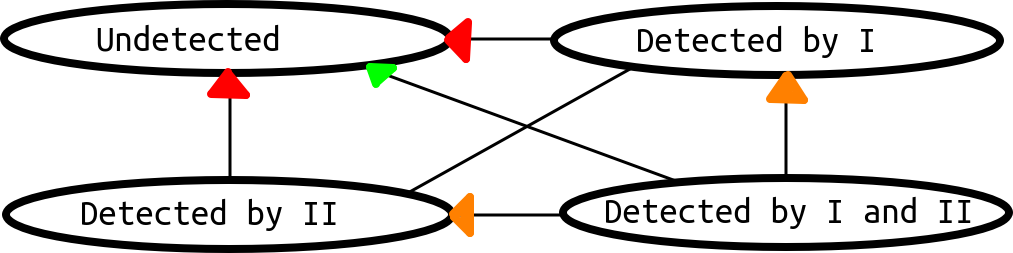
\includegraphics[width=\textwidth]{transitions.png}
  \caption{
    Transitions in TMHs that occur more often then expected by chance,
    for a confidence interval of 5 percent.
    Table \ref{tab:transitions} shows the transition counts.
    \richel{
      stub figure
    }
  }
  \label{fig:transitions}
\end{figure}

\begin{table}[!htbp]
  \input{table_transitions.latex}
  \caption{
    Transitions counts, where the row indicates the source state,
    and the column indicates the target state.
    First number per cell is the observed number of this state transition,
    where the second number is the expected number of this state transition
    as predicted by chance.
    An asterisk behind the observed count indicates that this count
    is unlikely to be caused by chance only.
    Figure \ref{fig:transitions} shows which transition counts are 
    unlikely to be caused by chance only.
  }
  \label{tab:transitions}
\end{table}

%%%%%%%%%%%%%%%%%%%%%%%%%%%%%%%%%%%%%%%%%%%%%%%%%%%%%%%%%%%%%%%%%%%%%%%%%%%%%%%%
\section{Conclusion}
%%%%%%%%%%%%%%%%%%%%%%%%%%%%%%%%%%%%%%%%%%%%%%%%%%%%%%%%%%%%%%%%%%%%%%%%%%%%%%%%

We found that the percentages of epitopes overlapping 
with TMHs for a human and viral proteome are 
[similar/different]. In other words, the
epitopes that MHC-I presents are [as/not as] likely 
to be derived from TMH within either a human host and its viral pathogen.

We found that the percentages of epitopes overlapping 
with TMHs for a human and bacterial proteome are 
[similar/different]. In other words, the
epitopes that MHC-I presents are [as/not as] likely 
to be derived from TMH within either a human host and its bacterial pathogen.

%%%%%%%%%%%%%%%%%%%%%%%%%%%%%%%%%%%%%%%%%%%%%%%%%%%%%%%%%%%%%%%%%%%%%%%%%%%%%%%%
\section{Discussion}
%%%%%%%%%%%%%%%%%%%%%%%%%%%%%%%%%%%%%%%%%%%%%%%%%%%%%%%%%%%%%%%%%%%%%%%%%%%%%%%%

We concluded that the
epitopes that MHC-I presents are [as/not as] likely 
to be derived from TMH within either a human host and its viral pathogen.
Because the full COVID-19 has 21 TMHs, the percentages
of MHC-I epitopes being part of a TMH are likelier to be affected by
stochasticity. We chose to use COVID-19 regardless, as the thousands
of its time-dated genomic sequences are ideal for determining the 
evolutionary conservation of MHC-I detecting TMHs. 

We concluded that the
epitopes that MHC-I presents are [as/not as] likely 
to be derived from TMH within either a human host and its bacterial pathogen.
Because a bacterium does not infect a cell, thus its polypeptides
will not be presented by MHC-I, this result is [unexpected/expected]

We aimed our evolutionary experiment at TMHs, because these can
be predicted well from a protein structure,
are common structures and are present in all pathogens. 
We could have done the same experiment on beta-turn,
as also these can be predicted well \cite{petersen2010netturnp},
are common structures and are present in all pathogens.

\richel{
  Note that most bacteria are opportunistic pathogens.
  Note that most bacteria are generalists.
  Note that most bacteria have different cell membranes (and walls), that
  may have different functional constraints than a human cell membrane
}

%%%%%%%%%%%%%%%%%%%%%%%%%%%%%%%%%%%%%%%%%%%%%%%%%%%%%%%%%%%%%%%%%%%%%%%%%%%%%%%%
\section{Acknowledgments}
%%%%%%%%%%%%%%%%%%%%%%%%%%%%%%%%%%%%%%%%%%%%%%%%%%%%%%%%%%%%%%%%%%%%%%%%%%%%%%%%

We thank the Center for Information Technology of the University 
of Groningen for its support and for providing access to the Peregrine 
high performance computing cluster. 

%%%%%%%%%%%%%%%%%%%%%%%%%%%%%%%%%%%%%%%%%%%%%%%%%%%%%%%%%%%%%%%%%%%%%%%%%%%%%%%%
\section{Data Accessibility}
%%%%%%%%%%%%%%%%%%%%%%%%%%%%%%%%%%%%%%%%%%%%%%%%%%%%%%%%%%%%%%%%%%%%%%%%%%%%%%%%

All code is archived at \url{http://github.com/richelbilderbeek/someplace},
with DOI \url{https://doi.org/12.3456/zenodo.1234567}.

%%%%%%%%%%%%%%%%%%%%%%%%%%%%%%%%%%%%%%%%%%%%%%%%%%%%%%%%%%%%%%%%%%%%%%%%%%%%%%%%
\section{Authors' contributions}
%%%%%%%%%%%%%%%%%%%%%%%%%%%%%%%%%%%%%%%%%%%%%%%%%%%%%%%%%%%%%%%%%%%%%%%%%%%%%%%%

RJCB and FB conceived the idea for this research. 
RJCB wrote the code.
RJCB and FB wrote the article.

%%%%%%%%%%%%%%%%%%%%%%%%%%%%%%%%%%%%%%%%%%%%%%%%%%%%%%%%%%%%%%%%%%%%%%%%%%%%%%%%
% Bibliography
%%%%%%%%%%%%%%%%%%%%%%%%%%%%%%%%%%%%%%%%%%%%%%%%%%%%%%%%%%%%%%%%%%%%%%%%%%%%%%%%
% MEE style
\bibliographystyle{mee}
\bibliography{article}
%%%%%%%%%%%%%%%%%%%%%%%%%%%%%%%%%%%%%%%%%%%%%%%%%%%%%%%%%%%%%%%%%%%%%%%%%%%%%%%%


%%%%%%%%%%%%%%%%%%%%%%%%%%%%%%%%%%%%%%%%%%%%%%%%%%%%%%%%%%%%%%%%%%%%%%%%%%%%%%%%
\appendix
\section{Supplementary materials}
%%%%%%%%%%%%%%%%%%%%%%%%%%%%%%%%%%%%%%%%%%%%%%%%%%%%%%%%%%%%%%%%%%%%%%%%%%%%%%%%

%%%%%%%%%%%%%%%%%%%%%%%%%%%%%%%%%%%%%%%%%%%%%%%%%%%%%%%%%%%%%%%%%%%%%%%%%%%%%%%%
\subsubsection{Fitness landscape}
\label{subsec:fitness_landscape}
%%%%%%%%%%%%%%%%%%%%%%%%%%%%%%%%%%%%%%%%%%%%%%%%%%%%%%%%%%%%%%%%%%%%%%%%%%%%%%%%

\paragraph{Introduction}
One could assume a two-state fitness landscape: being
undetected, due to zero epitopes, or being detected, due to one or more
epitopes. Alternatively, one may hypothesize a gradual fitness decrease per
extra epitope. Both fitness landscapes are depicted in 
figure \ref{fig:fitness_landscape}.

\begin{figure}[!htbp]
  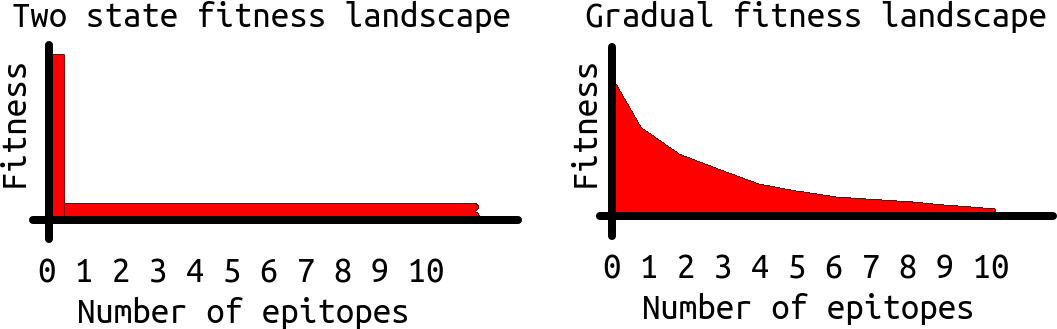
\includegraphics[width=\textwidth]{fitness_landscape.png}
  \caption{
    Two conceptual fitness landscapes. At the left is a two-state
    fitness landscape, in which the number of epitopes has a simple
    effect: a pathogen's fitness is high if it has no epitopes,
    as it is undetected by a host's immune system. 
    For one or more epitopes, fitness is at a same lower values. 
    In this fitness landscape, acquiring a second or third or more 
    epitope, this has no effect on fitness.
    At the right is a gradual fitness landscape, in which any increase in
    the number of epitopes results in a lower fitness.
  }
  \label{fig:fitness_landscape}
\end{figure}

\paragraph{Why}
This exploratory experiment tests an assumptions 
of the bigger evolutionary experiment. 
If the assumption is incorrect,
a different evolutionary experiment needs to be contrived.

\paragraph{Method}
For a given MHC-I haplotype, we count the number of epitopes in 
the proteome of COVID-19, at the start of the 2019 pandemic (as
described in \cite{wu2020new})
and a random strain sequenced most recently at the day of the experiment. 
Of both proteomes, we use use \verb;epitope-prediction; \cite{bianchi2017} 
to count the number of predicted binders for the HLA-A-02:01 haplotype.
We use that haplotype, as it is the haplotype used by default with the
\verb;epitope-prediction; package.

\paragraph{Decision rule}
If the number of epitopes has increased, we assume a two-state fitness landscape,
in which the number of epitopes can increase neutrally by drift alone.
In this case, the experiment will be cancelled and replaced by a 
viable approach.
Else, the bigger evolutionary experiment is done as described already.
It may still be possible that the number of epitopes decreased due to drift,
but this would be a proper result in confirming the null hypothesis
of $\mathcal{H}_{3,HVB}$.

\paragraph{Method detail}
Because the proteome is only sequenced at the start of the pandemic,
we use the DNA sequences of both strains, and infer the proteome
of each, using Prodigal. Although the earlier strand has a published
proteome, we infer it regardless, as to use the same pipeline.
If needed, we tweak the Prodigal parameter settings up until
the inferred proteome of the earlier strain with known proteome
matches well enough, as concluded by eyeballing.
The parameter settings used to infer a good proteome on the earlier
strain, is then used on the genome of the more recent strain 
to infer our recent proteome.

%%%%%%%%%%%%%%%%%%%%%%%%%%%%%%%%%%%%%%%%%%%%%%%%%%%%%%%%%%%%%%%%%%%%%%%%%%%%%%%%
\subsection{MHC-I}
%%%%%%%%%%%%%%%%%%%%%%%%%%%%%%%%%%%%%%%%%%%%%%%%%%%%%%%%%%%%%%%%%%%%%%%%%%%%%%%%

\begin{table}
  \input{bbbq_1/bbbq_1_percentages.latex}
  \caption{
    Percentage of MHC-I epitopes overlapping with transmembrane helix.
    \richel{This is simulated data}
  }
  \label{table:bbbq_1_percentages}
\end{table}

\begin{table}
  \input{bbbq_1/bbbq_1_stats_covid.latex}
  \caption{
    Kolmogorov-Smirnov test results comparing human and COVID-19 for MHC-I
    \richel{Done on the simulated data}
  }
  \label{table:bbbq_1_stats_covid}
\end{table}

\begin{table}
  \input{bbbq_1/bbbq_1_stats_myco.latex}
  \caption{
    Kolmogorov-Smirnov test results comparing human and Mycobacterium for MHC-I
    \richel{Done on the simulated data}
  }
  \label{table:bbbq_1_stats_myco}
\end{table}

%%%%%%%%%%%%%%%%%%%%%%%%%%%%%%%%%%%%%%%%%%%%%%%%%%%%%%%%%%%%%%%%%%%%%%%%%%%%%%%%
\subsection{MHC-II}
%%%%%%%%%%%%%%%%%%%%%%%%%%%%%%%%%%%%%%%%%%%%%%%%%%%%%%%%%%%%%%%%%%%%%%%%%%%%%%%%

\begin{table}
  \input{bbbq_2/bbbq_2_percentages.latex}
  \caption{
    Percentage of MHC-II epitopes overlapping with transmembrane helix.
    \richel{This is simulated data}
  }
  \label{table:bbbq_2_percentages}
\end{table}

\begin{table}
  \input{bbbq_2/bbbq_2_stats_covid.latex}
  \caption{
    Kolmogorov-Smirnov test results comparing human and COVID-19 for MHC-II
    \richel{Done on the simulated data}
  }
  \label{table:bbbq_2_stats_covid}
\end{table}

\begin{table}
  \input{bbbq_2/bbbq_2_stats_myco.latex}
  \caption{
    Kolmogorov-Smirnov test results comparing human and Mycobacterium for MHC-II
    \richel{Done on the simulated data}
  }
  \label{table:bbbq_2_stats_myco}
\end{table}

%%%%%%%%%%%%%%%%%%%%%%%%%%%%%%%%%%%%%%%%%%%%%%%%%%%%%%%%%%%%%%%%%%%%%%%%%%%%%%%%
\subsection{COVID-19 genome and proteome}
%%%%%%%%%%%%%%%%%%%%%%%%%%%%%%%%%%%%%%%%%%%%%%%%%%%%%%%%%%%%%%%%%%%%%%%%%%%%%%%%

Tip: see \cite{bar2020sars} for COVID-19 in numbers.

\richel{
  This is just a reminder, instead of new research. 
  This subsection be deleted in the future.
}

\begin{figure}[!htbp]
  \includegraphics[width=0.9\textwidth]{pics/covid_genome_and_proteome.png}
  \caption{
    Overview of COVID-19 genome and proteome.
    From 
    \url{https://zhanglab.ccmb.med.umich.edu/COVID-19}
  }
  \label{fig:covid_genome_and_proteome}
\end{figure}

%%%%%%%%%%%%%%%%%%%%%%%%%%%%%%%%%%%%%%%%%%%%%%%%%%%%%%%%%%%%%%%%%%%%%%%%%%%%%%%%
\subsection{Relation between hydrophobicity, TMH and MHC binding}
%%%%%%%%%%%%%%%%%%%%%%%%%%%%%%%%%%%%%%%%%%%%%%%%%%%%%%%%%%%%%%%%%%%%%%%%%%%%%%%%

\begin{figure}[!htbp]
  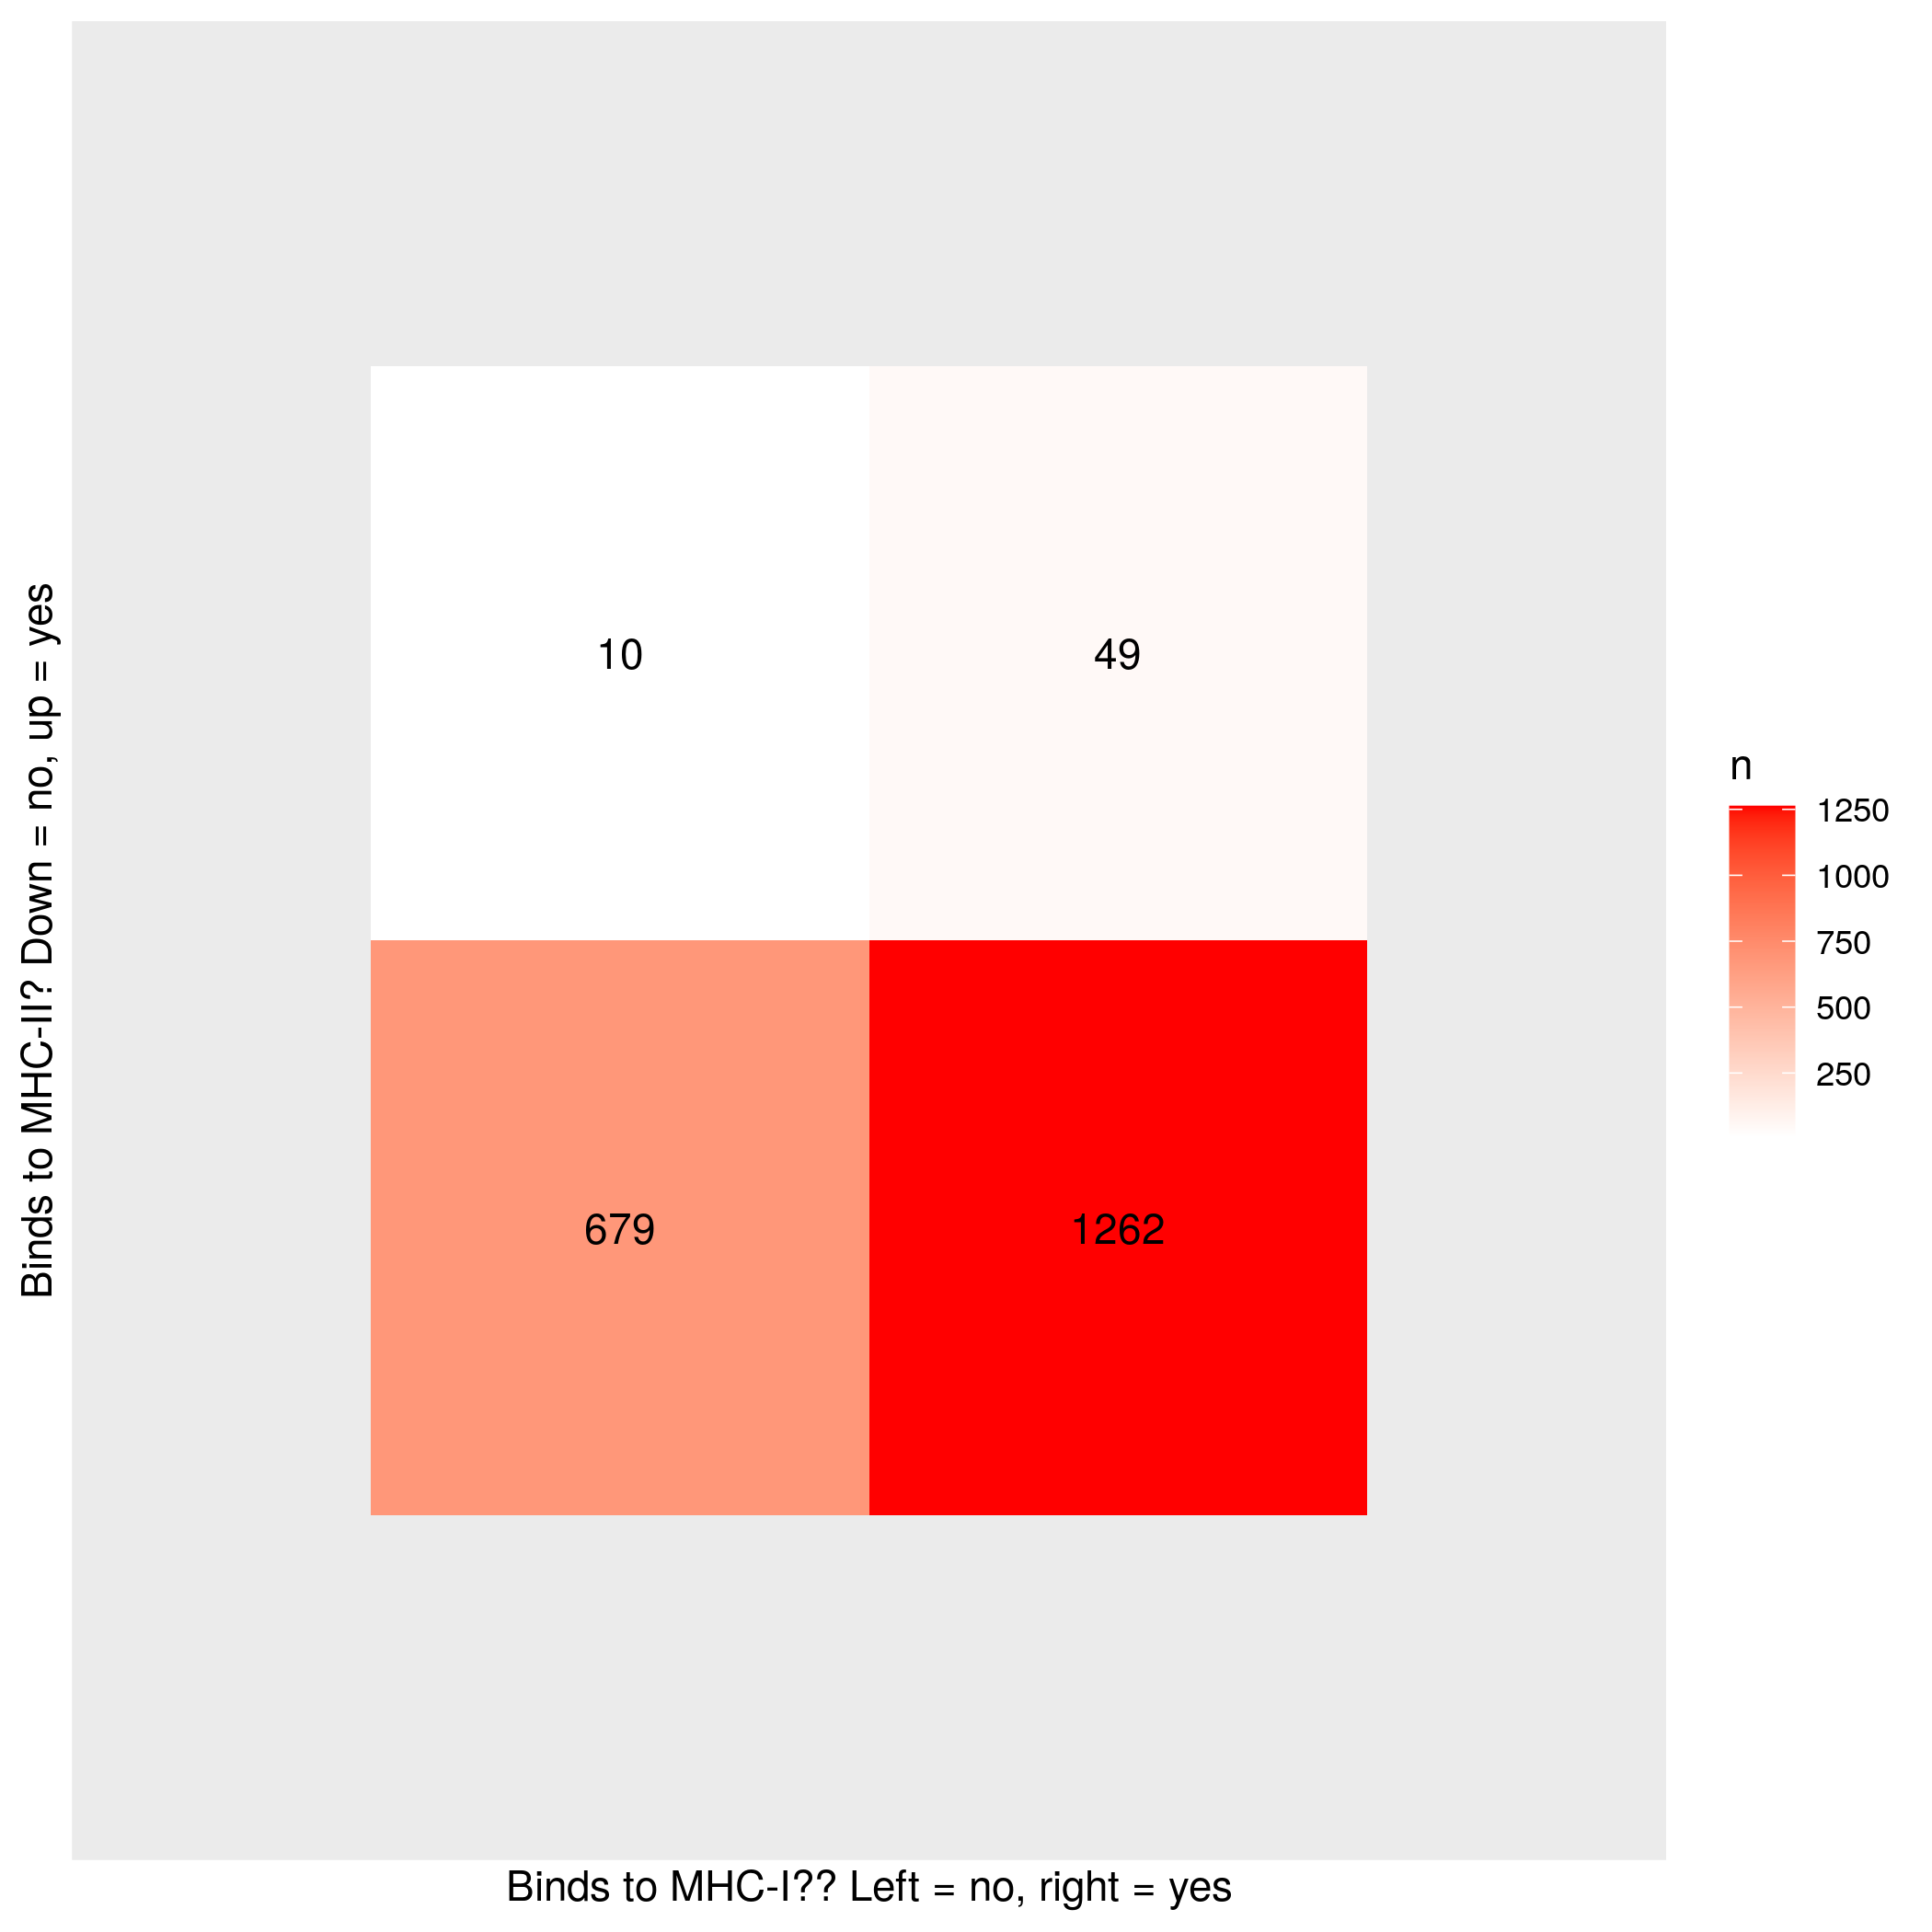
\includegraphics[width=0.9\textwidth]{p_bind_per_hydrophobicity/binds_mhc1_vs_binds_mhc2.png}
  \caption{
    \richel{Used randomly simulated polypeptides, results are real}
  }
  \label{fig:binds_mhc1_vs_binds_mhc2}
\end{figure}

\begin{figure}[!htbp]
  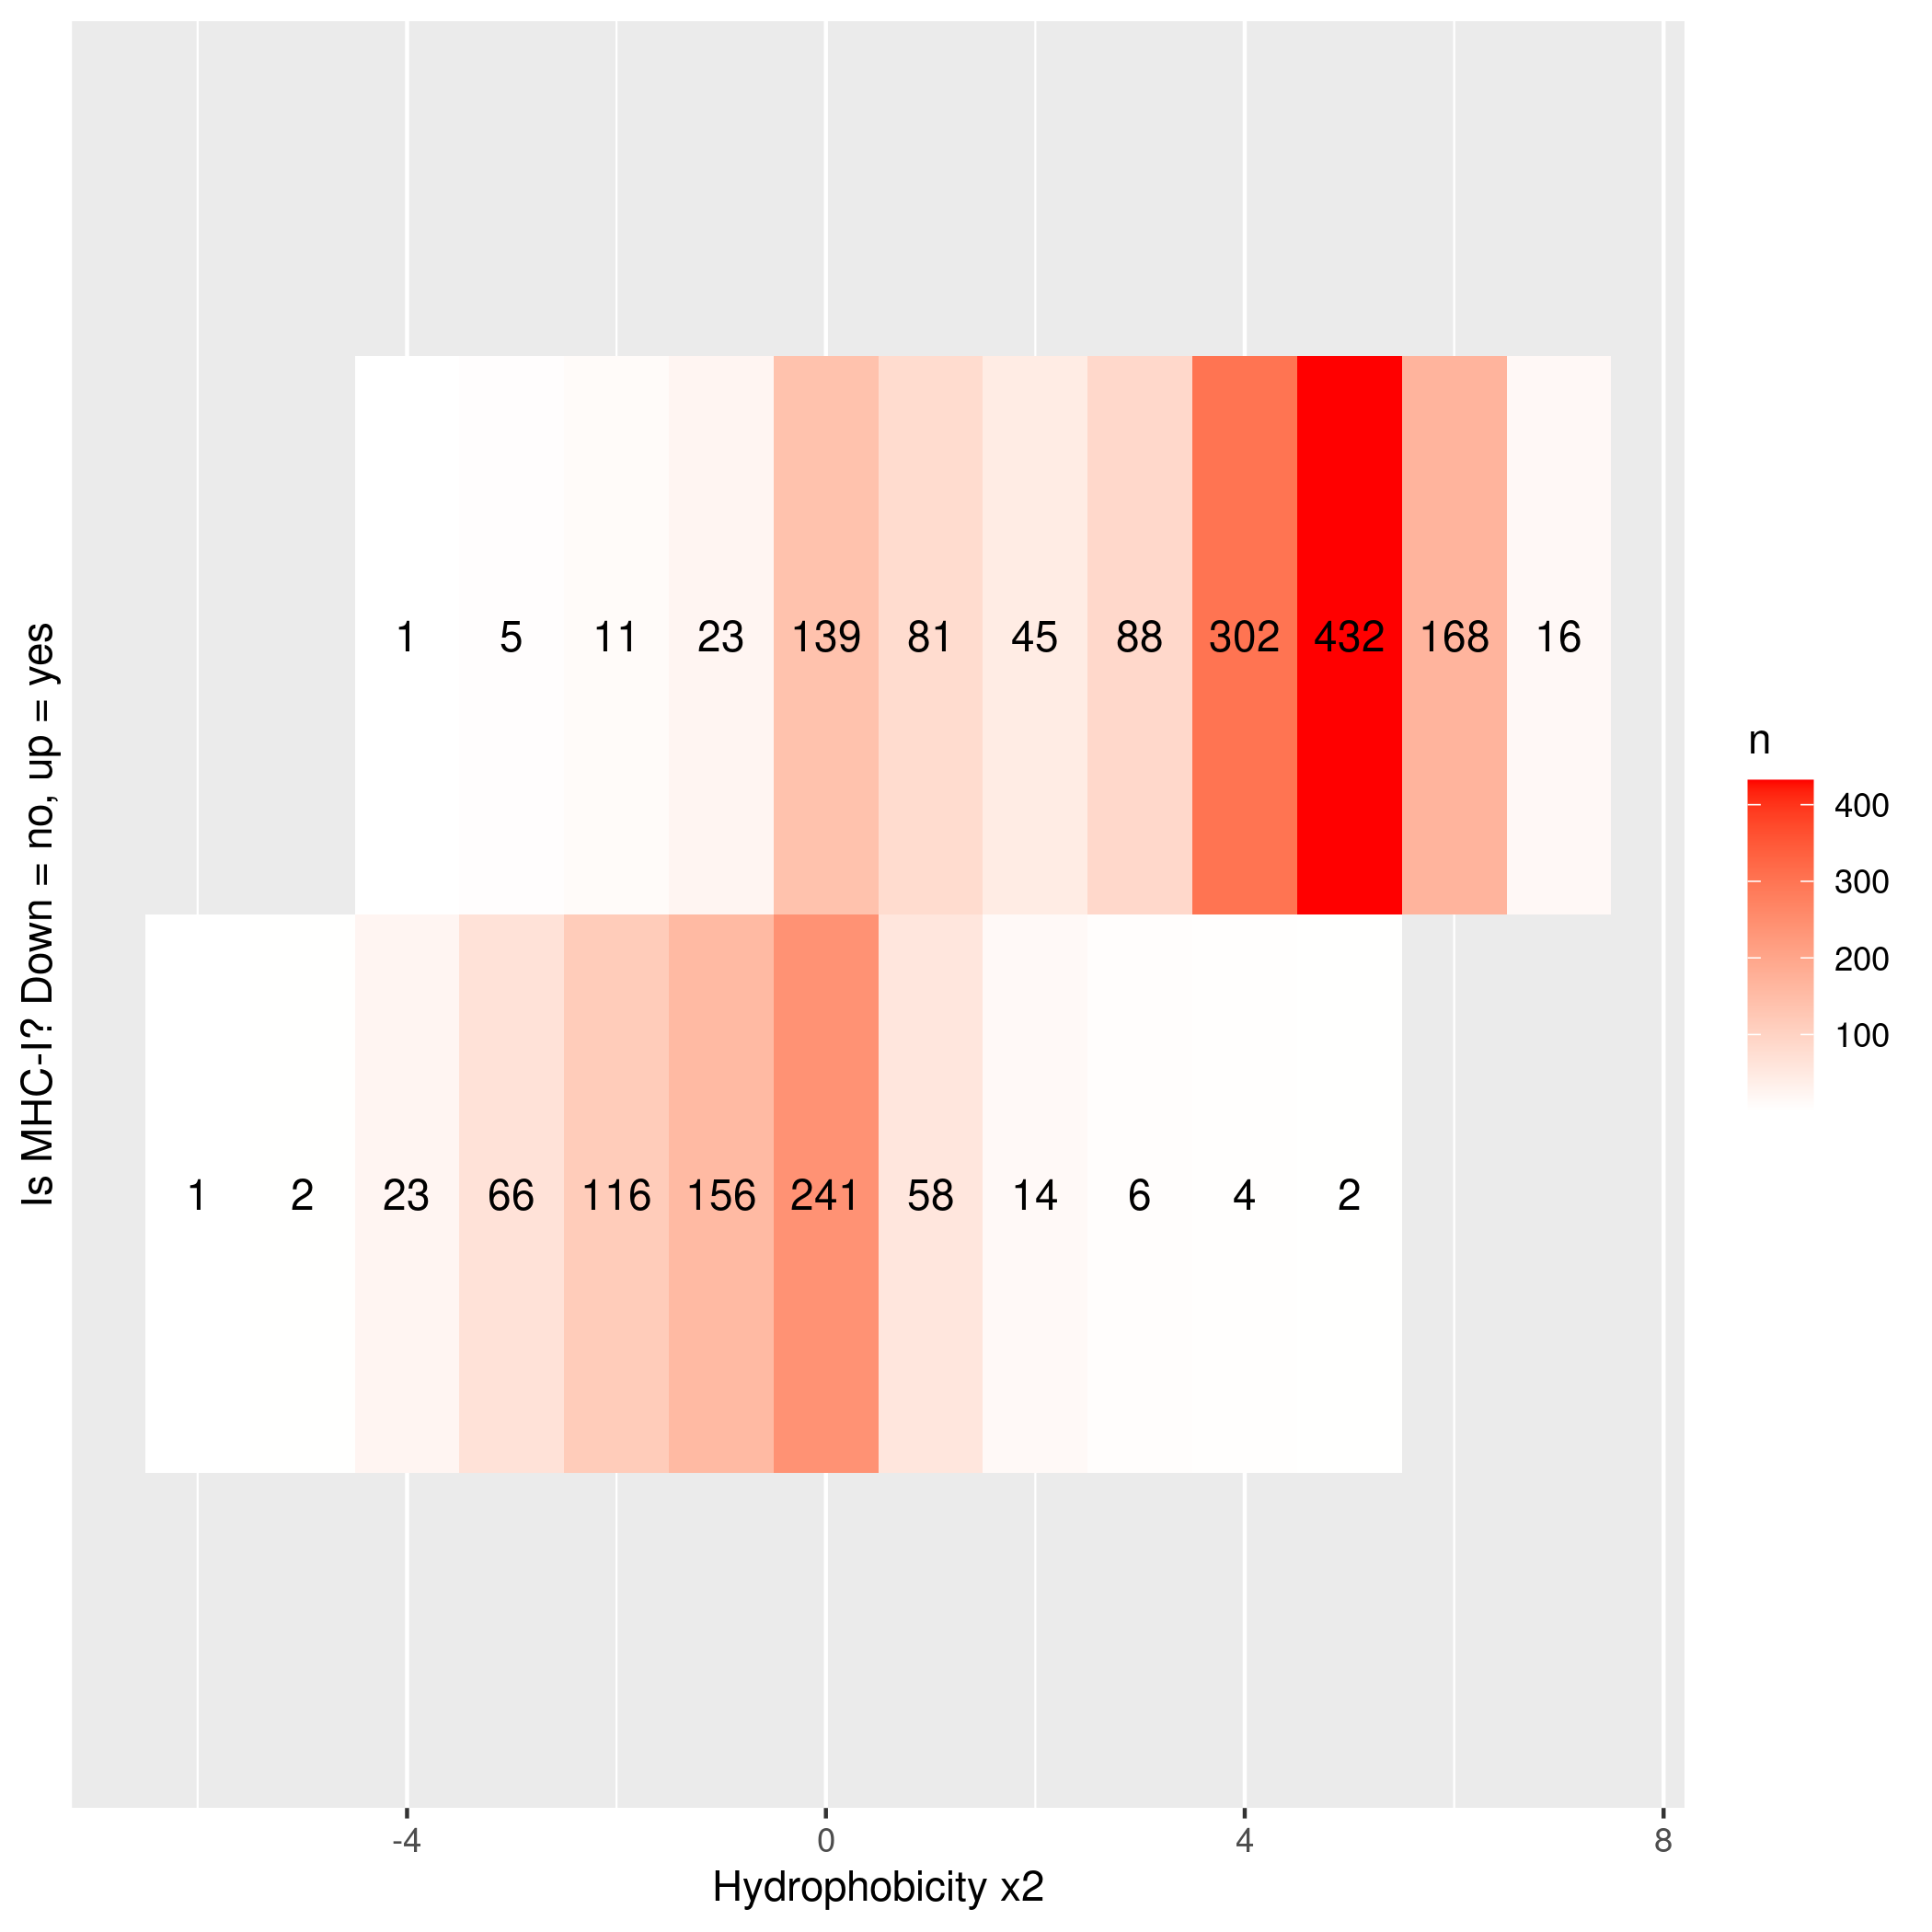
\includegraphics[width=0.9\textwidth]{p_bind_per_hydrophobicity/hydrophobicity_vs_binds_mhc1.png}
  \caption{
    \richel{Used randomly simulated polypeptides, results are real}
  }
  \label{fig:hydrophobicity_vs_binds_mhc1}
\end{figure}

\begin{figure}[!htbp]
  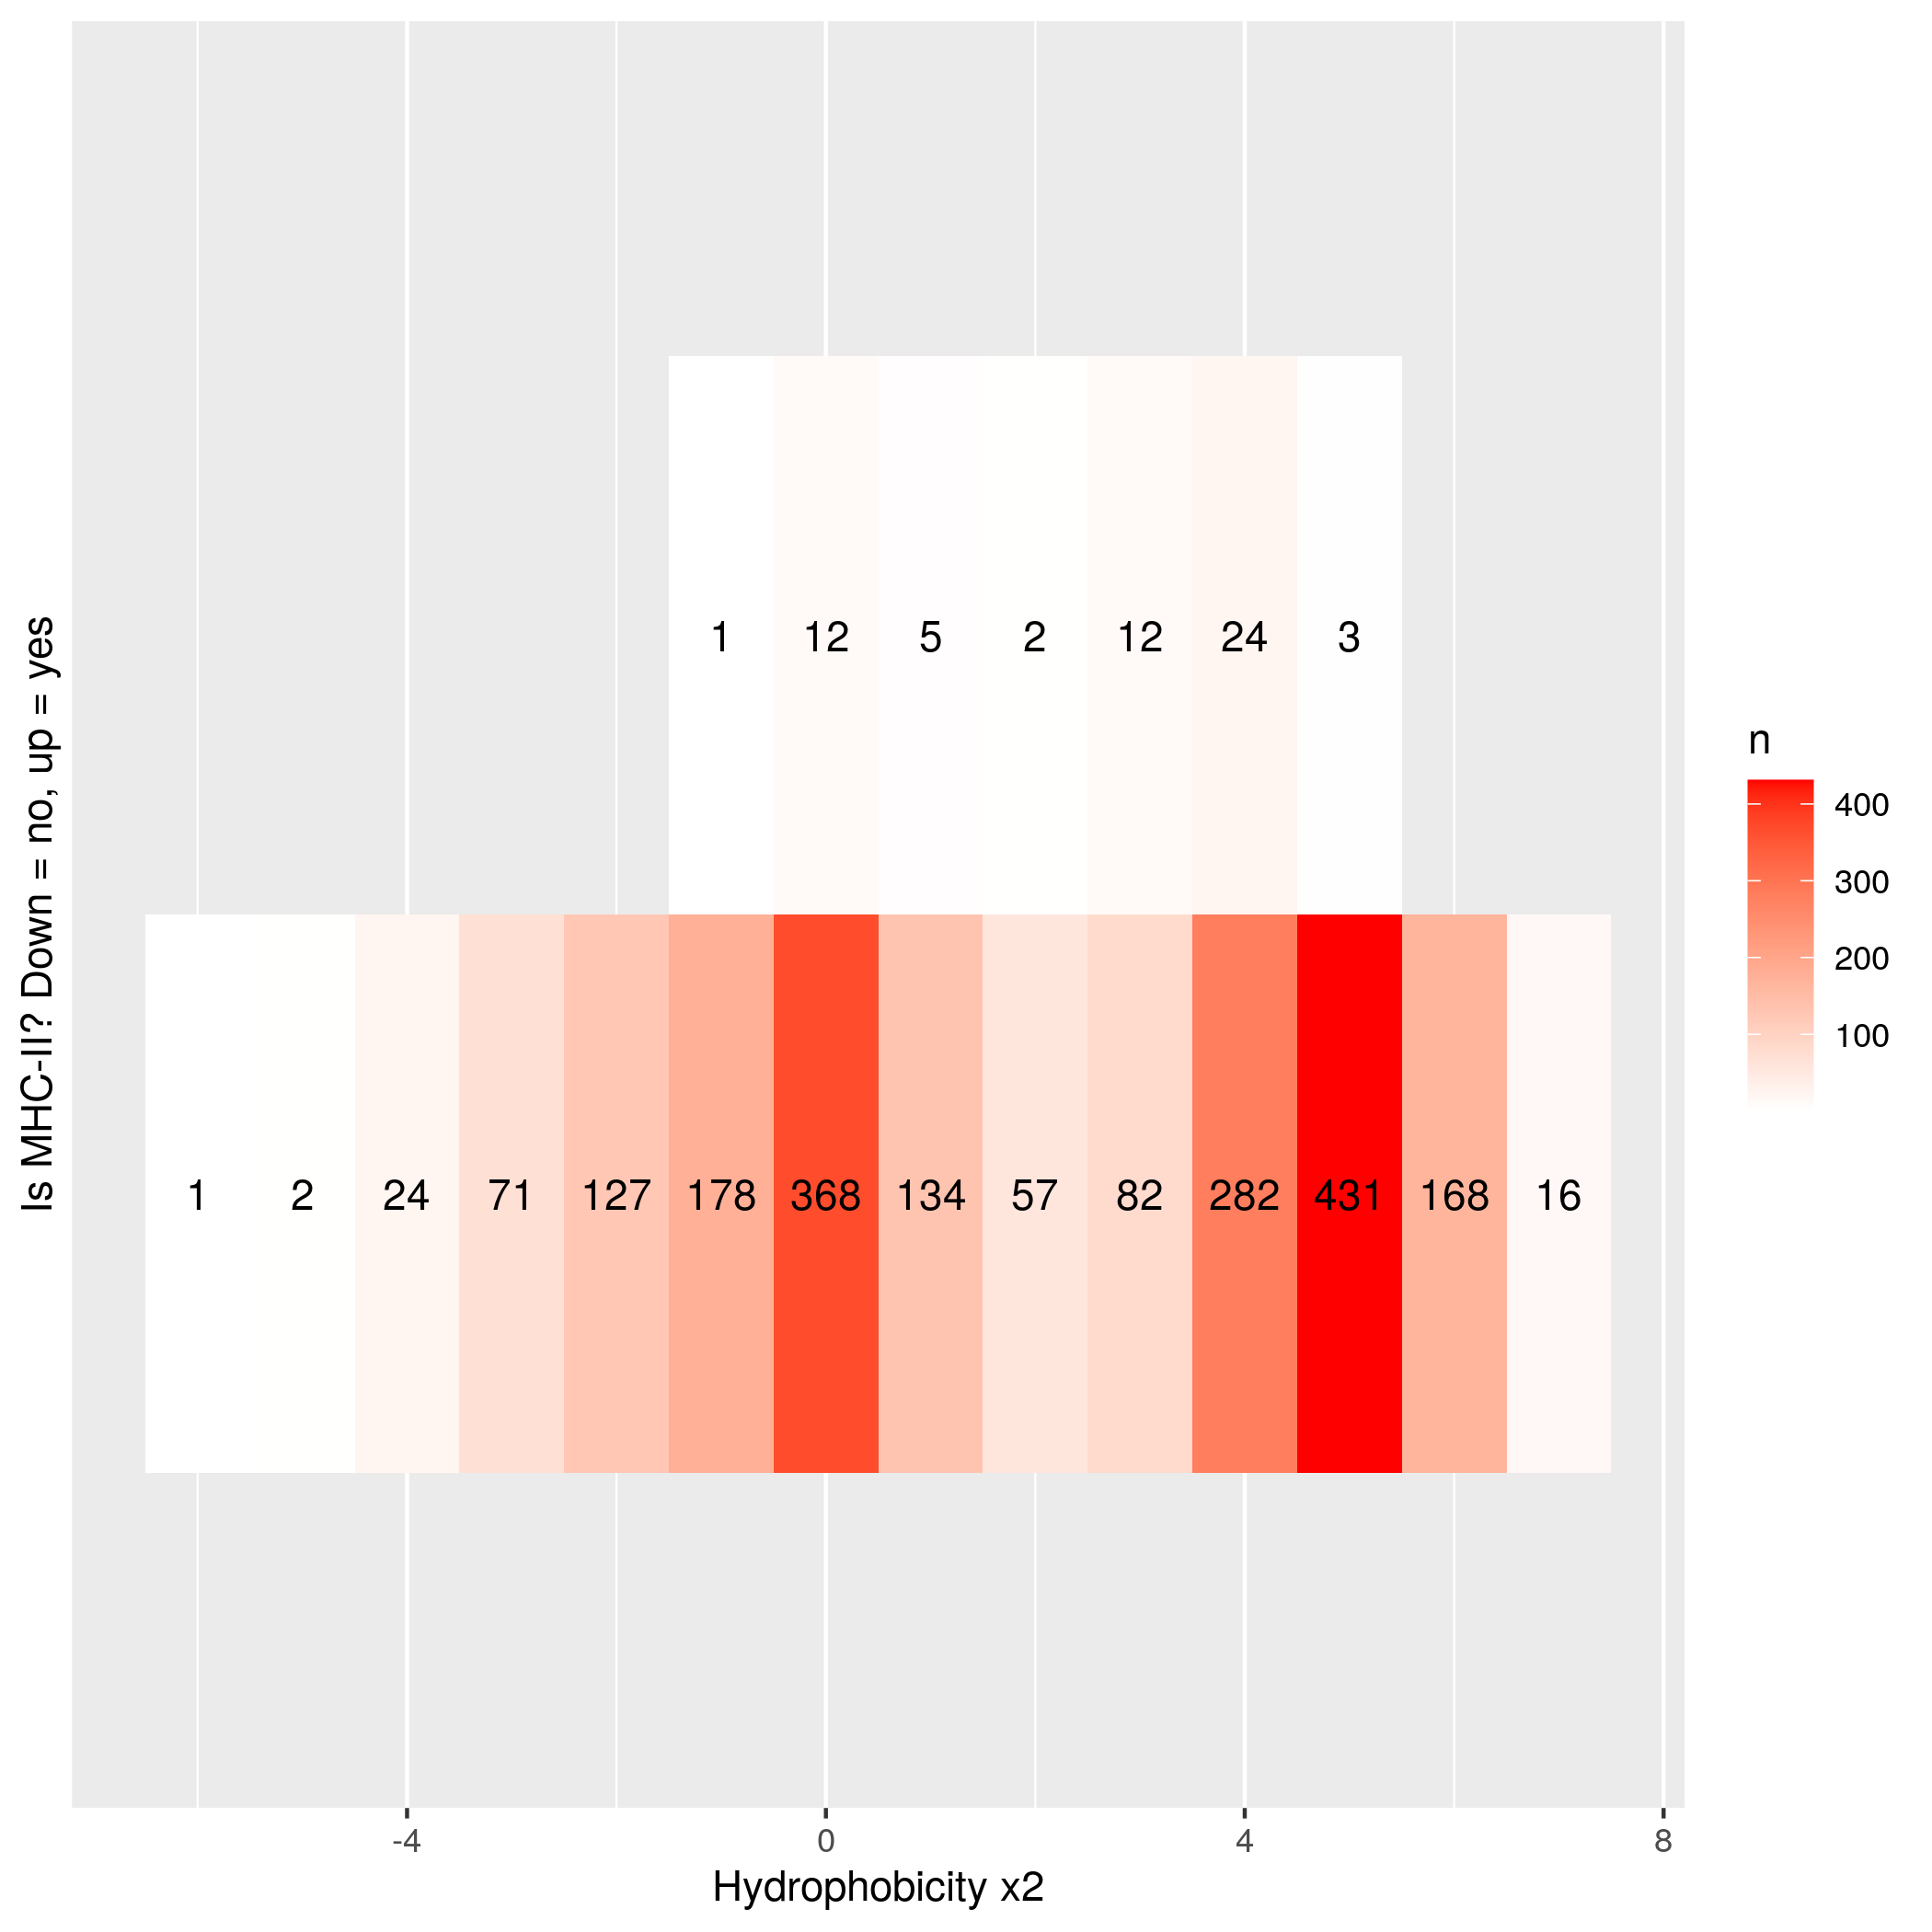
\includegraphics[width=0.9\textwidth]{p_bind_per_hydrophobicity/hydrophobicity_vs_binds_mhc2.png}
  \caption{
    \richel{Used randomly simulated polypeptides, results are real}
  }
  \label{fig:hydrophobicity_vs_binds_mhc2}
\end{figure}

\begin{figure}[!htbp]
  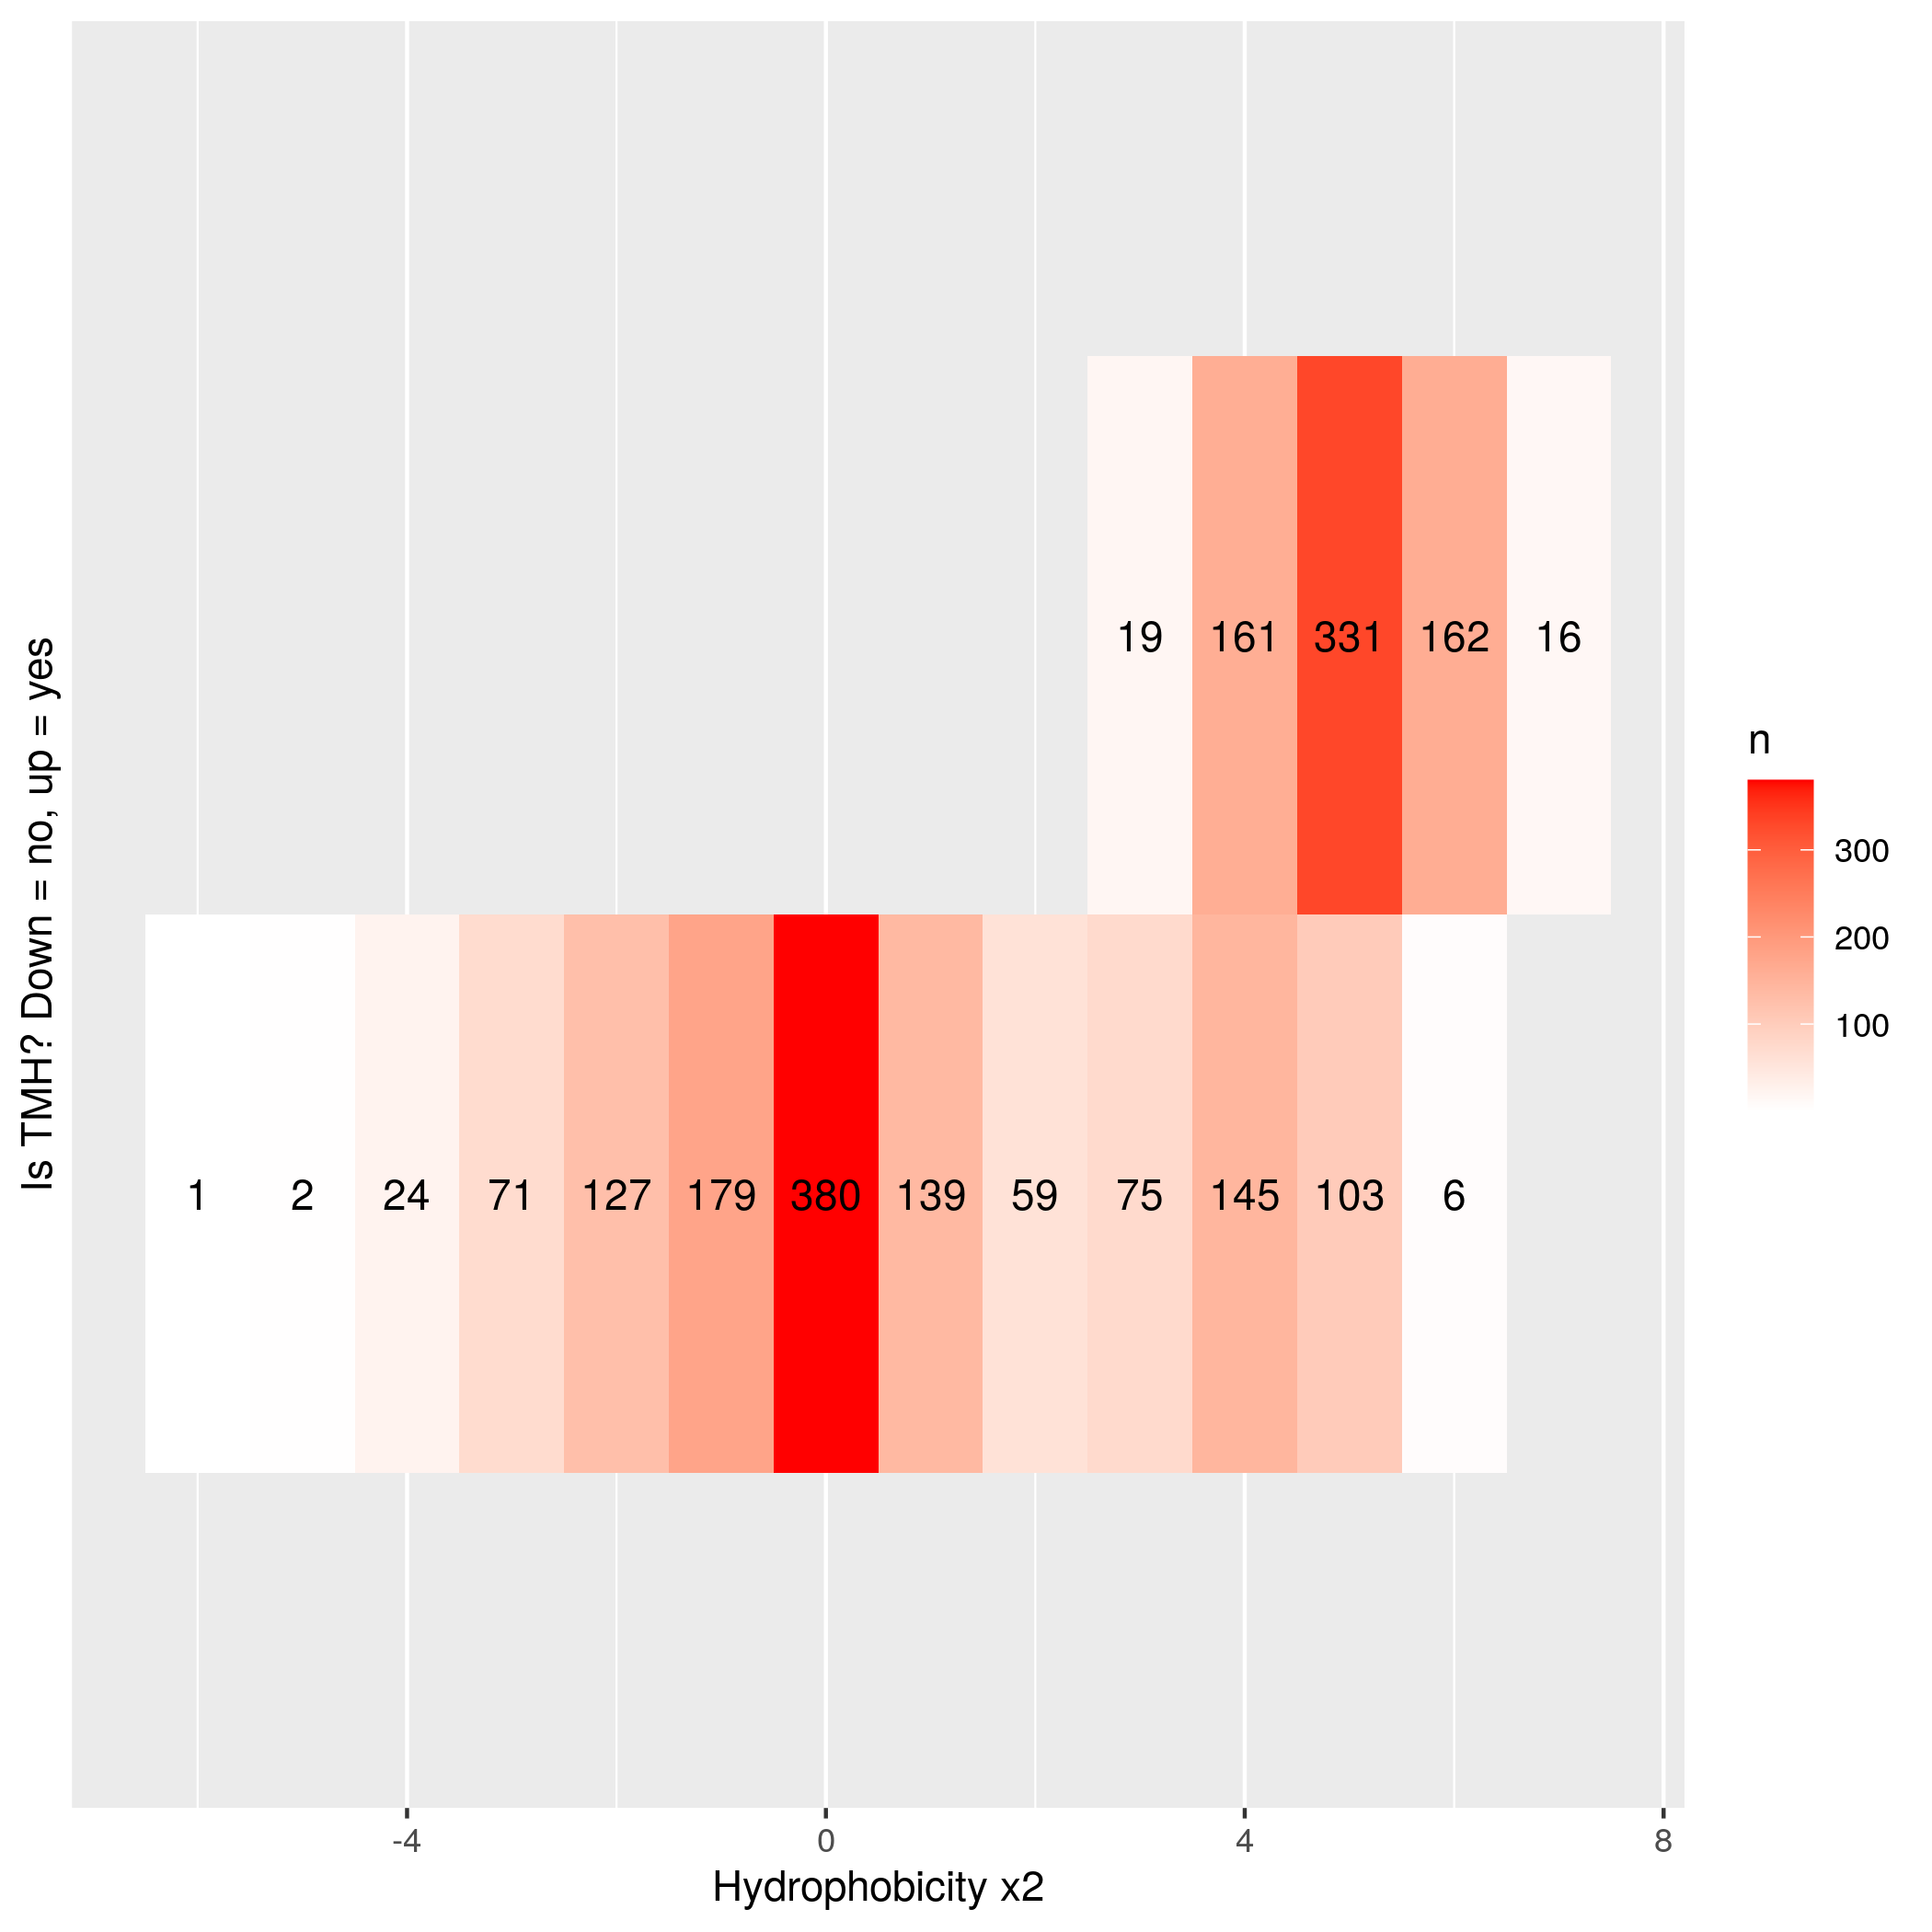
\includegraphics[width=0.9\textwidth]{p_bind_per_hydrophobicity/hydrophobicity_vs_is_tmh.png}
  \caption{
    \richel{Used randomly simulated polypeptides, results are real}
  }
  \label{fig:hydrophobicity_vs_is_tmh}
\end{figure}

\begin{figure}[!htbp]
  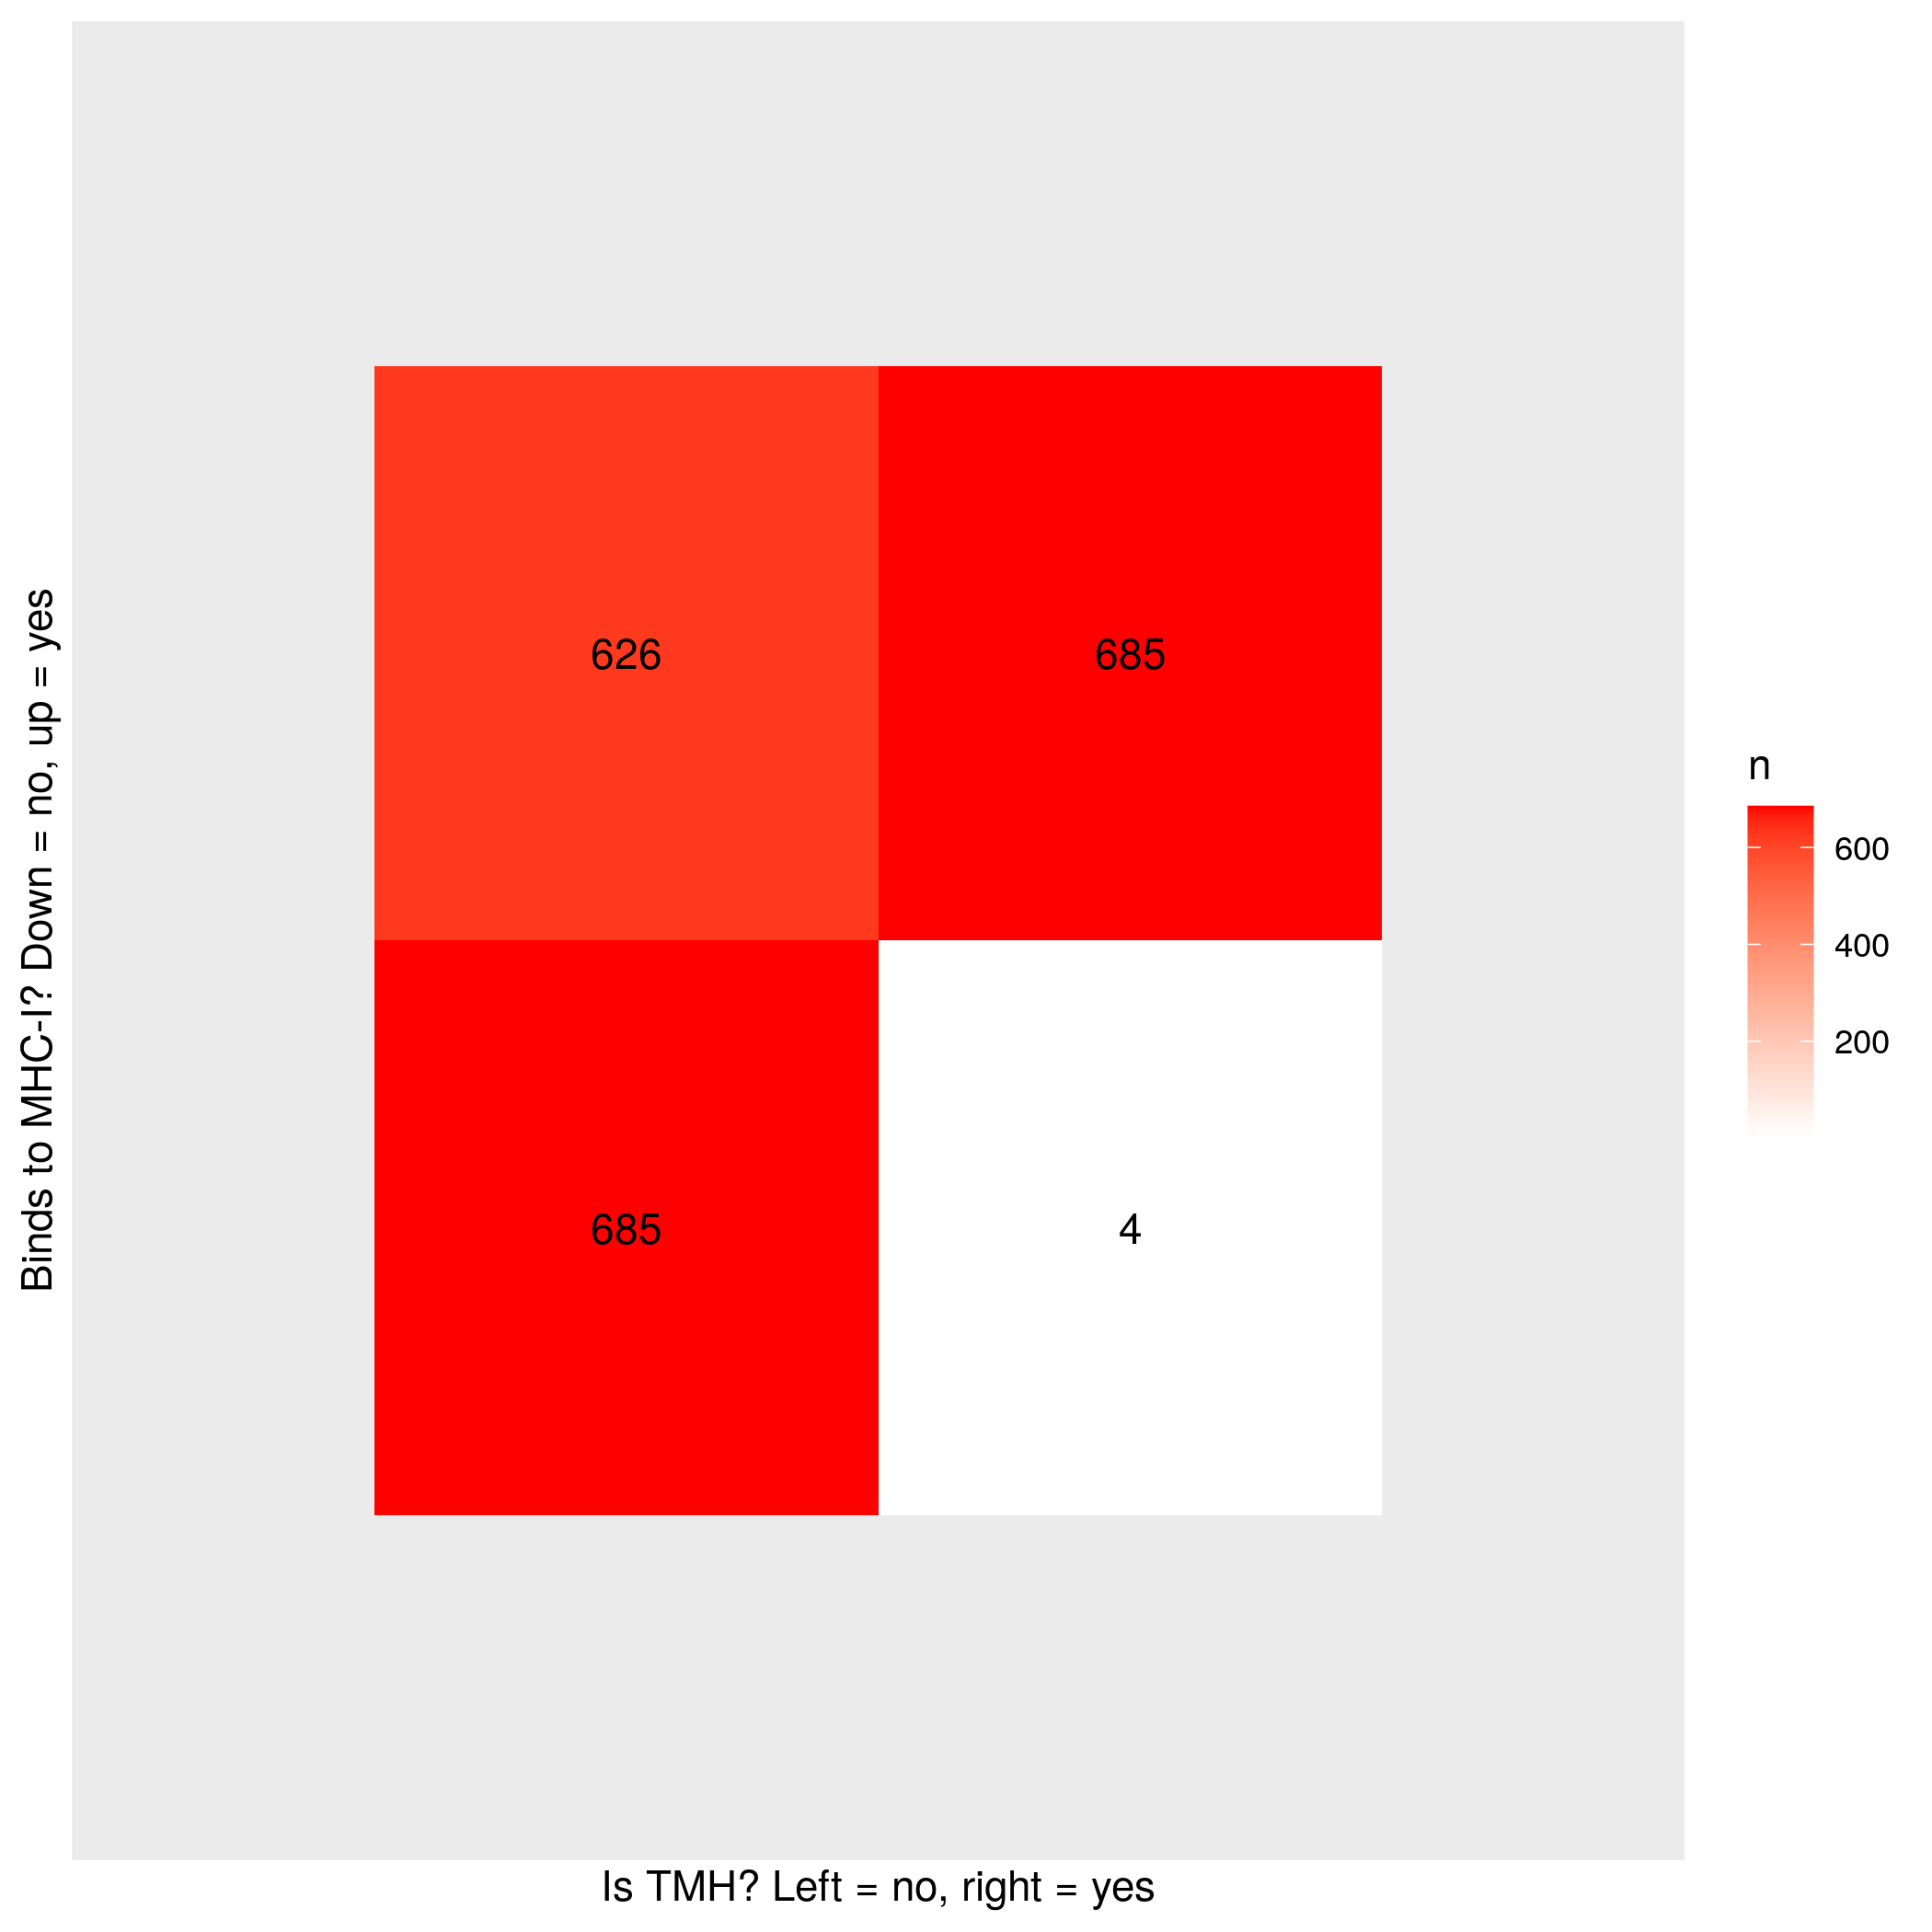
\includegraphics[width=0.9\textwidth]{p_bind_per_hydrophobicity/is_tmh_vs_binds_mhc1.png}
  \caption{
    \richel{Used randomly simulated polypeptides, results are real}
  }
  \label{fig:is_tmh_vs_binds_mhc1}
\end{figure}

\begin{figure}[!htbp]
  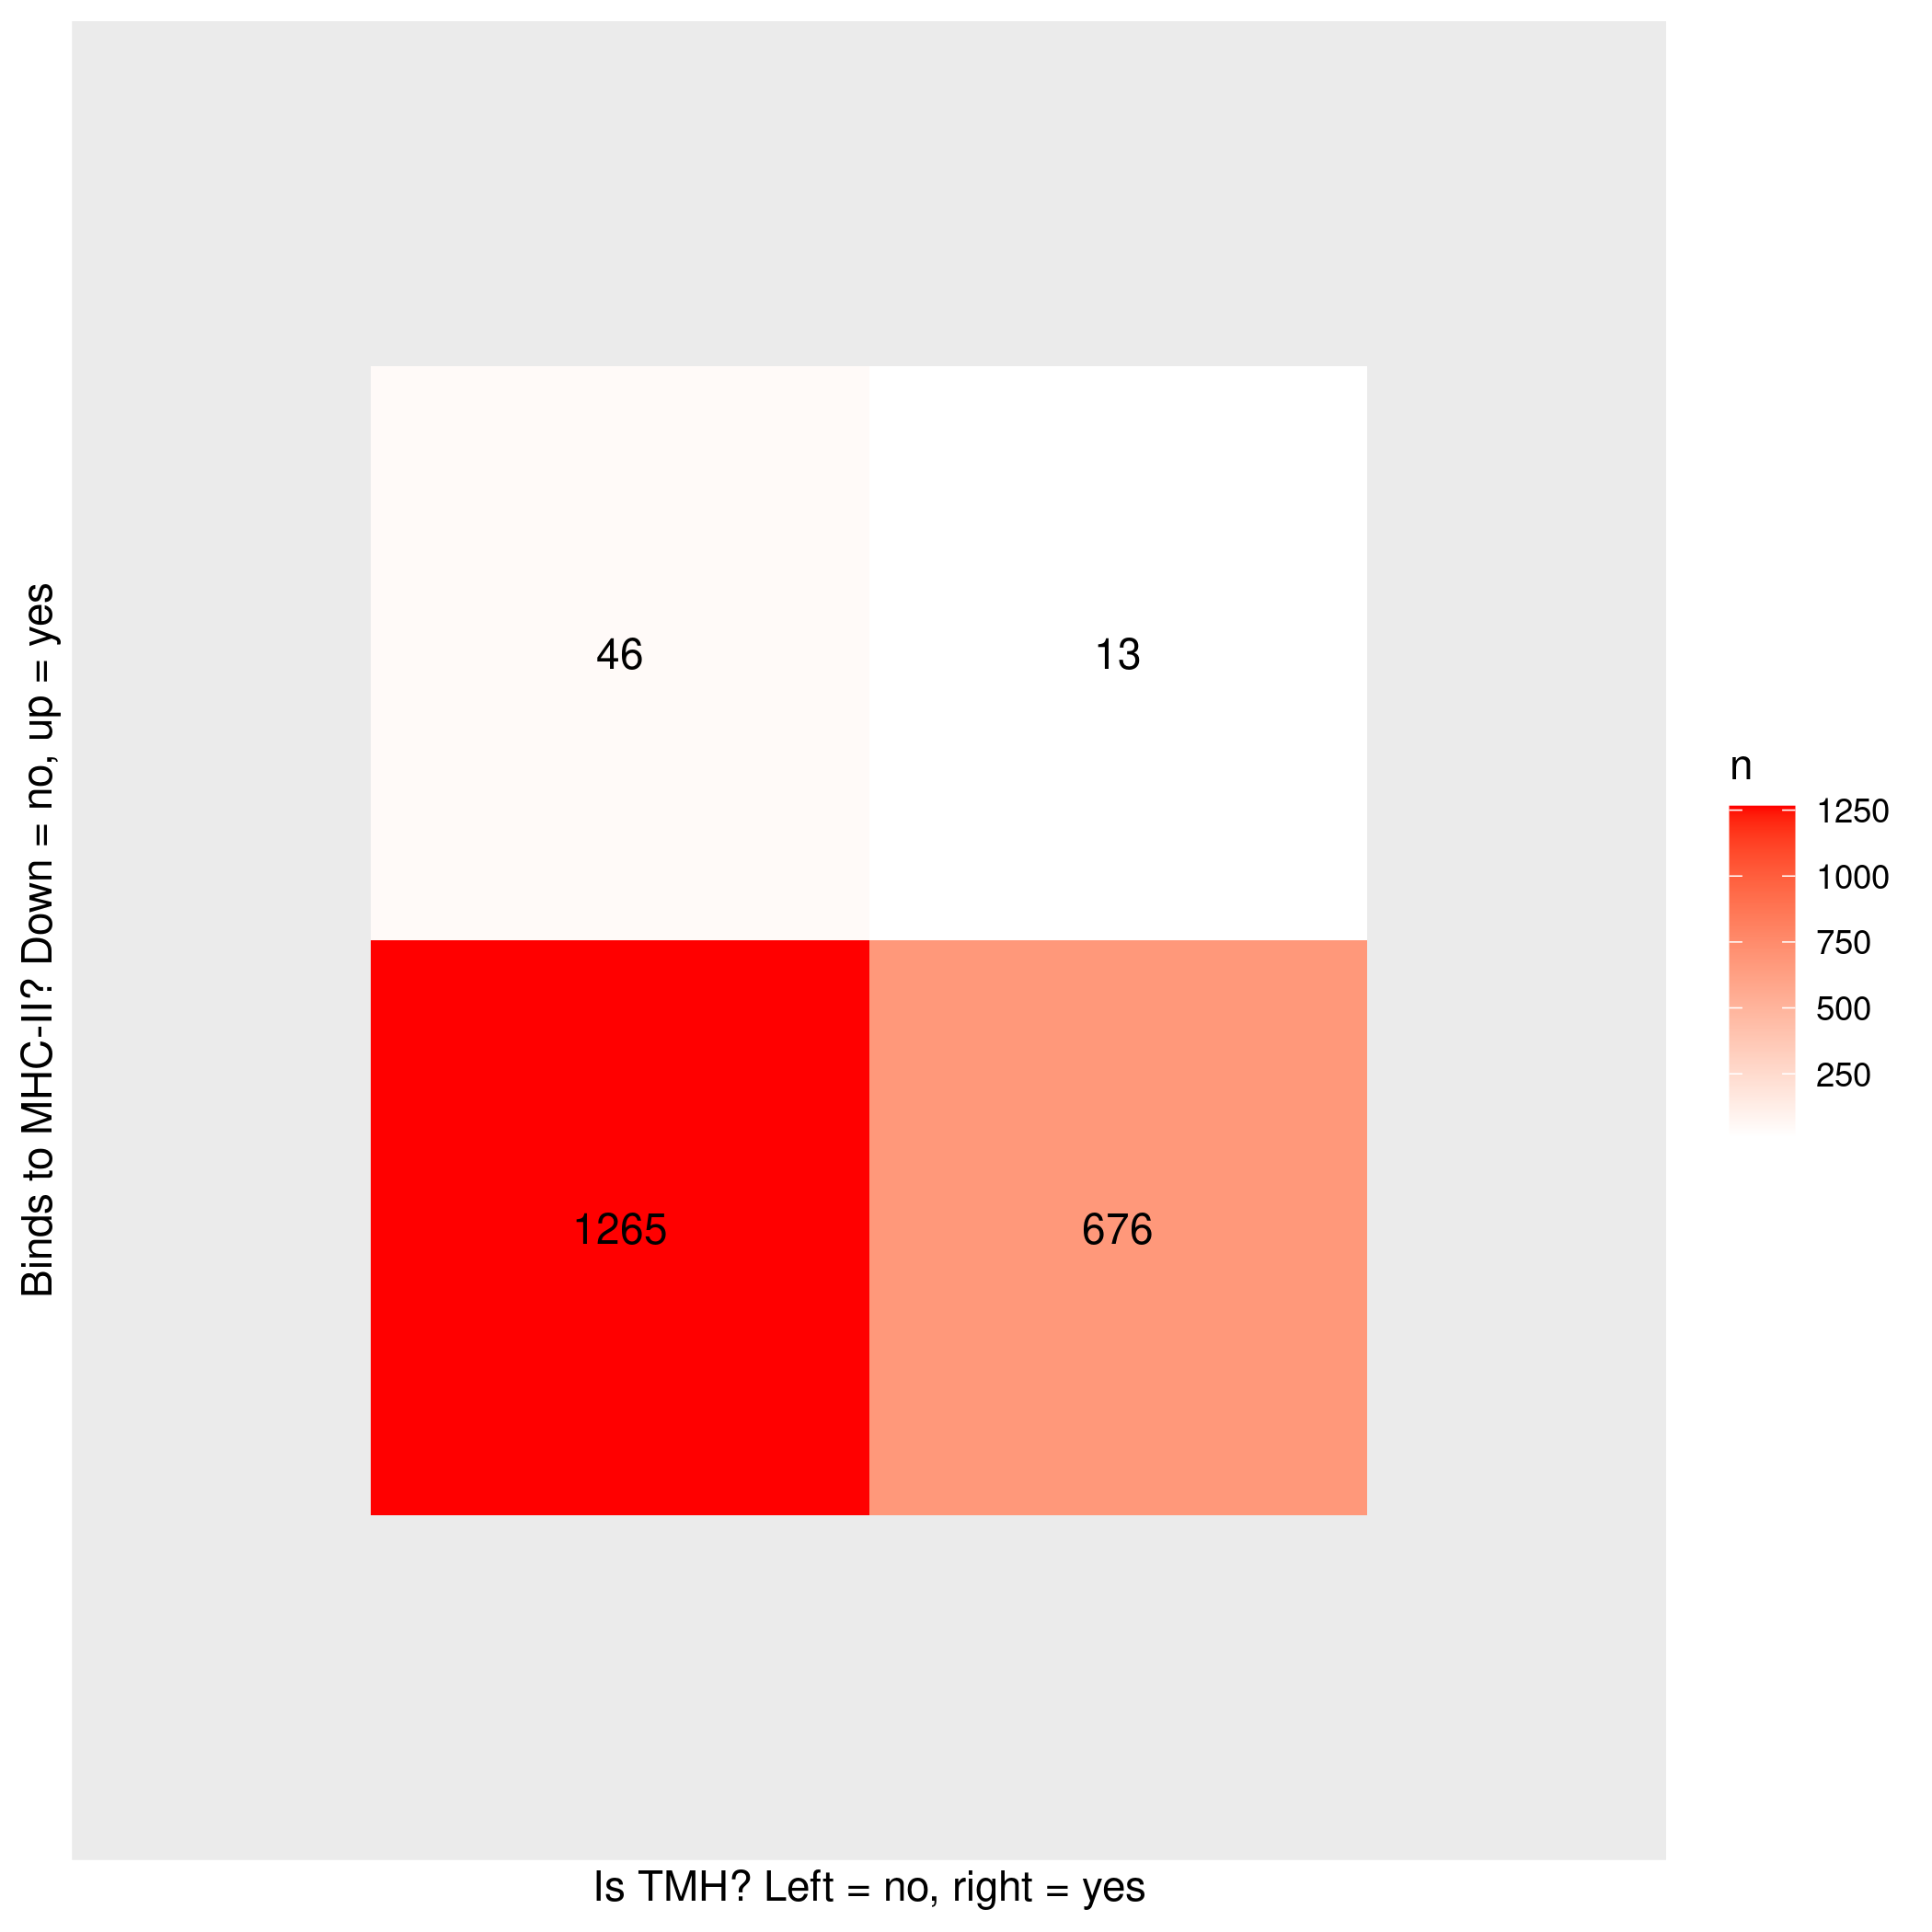
\includegraphics[width=0.9\textwidth]{p_bind_per_hydrophobicity/is_tmh_vs_binds_mhc2.png}
  \caption{
    \richel{Used randomly simulated polypeptides, results are real}
  }
  \label{fig:is_tmh_vs_binds_mhc2}
\end{figure}


%%%%%%%%%%%%%%%%%%%%%%%%%%%%%%%%%%%%%%%%%%%%%%%%%%%%%%%%%%%%%%%%%%%%%%%%%%%%%%%%
\subsection{COVID-19 TMHs}
%%%%%%%%%%%%%%%%%%%%%%%%%%%%%%%%%%%%%%%%%%%%%%%%%%%%%%%%%%%%%%%%%%%%%%%%%%%%%%%%

\begin{figure}[!htbp]
  \includegraphics[width=\textwidth]{tmhs/tmhs.png}
  \caption{
    Location of amino acids of reference COVID-19 proteome.
    Note that ORF1a results in multiple proteins, 
    as shown in figure \ref{fig:covid_genome_and_proteome}.
    Legend: i = inside (cytosolic side), m = membrane, o = outside (extracellular side)
    \richel{This is real data}
  }
  \label{fig:covid_locatome}
\end{figure}


%%%%%%%%%%%%%%%%%%%%%%%%%%%%%%%%%%%%%%%%%%%%%%%%%%%%%%%%%%%%%%%%%%%%%%%%%%%%%%%%
\subsection{MHC-II haplotype occurrences}
%%%%%%%%%%%%%%%%%%%%%%%%%%%%%%%%%%%%%%%%%%%%%%%%%%%%%%%%%%%%%%%%%%%%%%%%%%%%%%%%

\richel{
  This is just a reminder, instead of new research. 
  This subsection be deleted in the future.
}

\begin{table}
  \input{mhc2_haplotypes.latex}
  \caption{
    Percentage of MHC-II haplotypes, from \cite{greenbaum2011functional}
    \richel{
      This is just a reminder, instead of new research. 
      This table be deleted in the future.
    }
  }
  \label{table:mhc2_haplotypes}
\end{table}

%%%%%%%%%%%%%%%%%%%%%%%%%%%%%%%%%%%%%%%%%%%%%%%%%%%%%%%%%%%%%%%%%%%%%%%%%%%%%%%%
\subsection{Kolmogorov-Smirnov}
%%%%%%%%%%%%%%%%%%%%%%%%%%%%%%%%%%%%%%%%%%%%%%%%%%%%%%%%%%%%%%%%%%%%%%%%%%%%%%%%

\richel{
  This is just a reminder, instead of new research. 
  This subsection be deleted in the future.
}

The Kolmogorov-Smirnov (KS) test determines if two samples
are derived from the same distribution, without making assumptions
regarding the shape of that distribution. 

We will reject
the null hypothesis that MHC-I has the same percentage of epitopes 
overlapping with TMHs in Homo sapiens compared to each pathogen when 
the KS statistic $D_{n,m}$ follows the relationship as shown in 
equation \ref{eq:ks}, for a significance level $\alpha = 0.05$
and $n = m$ equals the number of HLA haplotypes.

\begin{equation}
   D_{n,m} > \frac{1}{\sqrt{n}} \cdot \sqrt{ -\ln(\frac{\alpha}{2}) \cdot \frac{1 + \frac{n}{m}}{2} }
   \label{eq:ks}
\end{equation}

\end{document}
new research. 
      This table be deleted in the future.
    }
  }
  \label{table:mhc2_haplotypes}
\end{table}

%%%%%%%%%%%%%%%%%%%%%%%%%%%%%%%%%%%%%%%%%%%%%%%%%%%%%%%%%%%%%%%%%%%%%%%%%%%%%%%%
\subsection{Kolmogorov-Smirnov}
%%%%%%%%%%%%%%%%%%%%%%%%%%%%%%%%%%%%%%%%%%%%%%%%%%%%%%%%%%%%%%%%%%%%%%%%%%%%%%%%

\richel{
  This is just a reminder, instead of new research. 
  This subsection be deleted in the future.
}

The Kolmogorov-Smirnov (KS) test determines if two samples
are derived from the same distribution, without making assumptions
regarding the shape of that distribution. 

We will reject
the null hypothesis that MHC-I has the same percentage of epitopes 
overlapping with TMHs in Homo sapiens compared to each pathogen when 
the KS statistic $D_{n,m}$ follows the relationship as shown in 
equation \ref{eq:ks}, for a significance level $\alpha = 0.05$
and $n = m$ equals the number of HLA haplotypes.

\begin{equation}
   D_{n,m} > \frac{1}{\sqrt{n}} \cdot \sqrt{ -\ln(\frac{\alpha}{2}) \cdot \frac{1 + \frac{n}{m}}{2} }
   \label{eq:ks}
\end{equation}

\end{document}
